% ==============================================================================
% Journal Paper: Offensive Language Detection in Tamil Social Media Text
%               Using Multilingual Transformers — A Comparative Study
% ==============================================================================
% Single-column journal format, 12pt, ~21+ pages
% ==============================================================================

\documentclass[12pt, a4paper]{article}

% ── Packages ──────────────────────────────────────────────────────────────────
\usepackage[utf8]{inputenc}
\usepackage[T1]{fontenc}
\usepackage{mathptmx}                     % Times New Roman font
\usepackage[margin=2.5cm]{geometry}        % Standard journal margins
\usepackage{setspace}                      % Line spacing
\usepackage{graphicx}                      % Figures
\usepackage{booktabs}                      % Professional tables
\usepackage{tabularx}                      % Flexible-width tables
\usepackage{multirow}                      % Multi-row cells
\usepackage{array}                         % Table column formatting
\usepackage{amsmath,amssymb}               % Math
\usepackage{hyperref}                      % Clickable links
\usepackage{xcolor}                        % Colors
\usepackage{float}                         % Float control
\usepackage{placeins}                      % \FloatBarrier
\usepackage{caption}                       % Caption formatting
\usepackage{subcaption}                    % Sub-figures
\usepackage{enumitem}                      % List formatting
\usepackage{tikz}                          % Architecture diagram
\usetikzlibrary{shapes.geometric, arrows.meta, positioning, fit, calc, backgrounds}
\usepackage{natbib}                        % Bibliography
\usepackage{url}                           % URL formatting
\usepackage{fancyhdr}                      % Headers/footers
\usepackage{titlesec}                      % Section formatting

% ── Settings ──────────────────────────────────────────────────────────────────
\onehalfspacing                            % 1.5 line spacing (journal standard)
\setlength{\parindent}{1.2em}
\setlength{\parskip}{0.3em}
\renewcommand{\arraystretch}{1.35}         % Table row spacing
\setlength{\tabcolsep}{8pt}               % Table column spacing

% Caption styling
\captionsetup{font=small, labelfont=bf, skip=8pt}
\captionsetup[table]{position=top}
\captionsetup[figure]{position=bottom}

% Hyperlink styling
\hypersetup{
    colorlinks=true,
    linkcolor=blue!70!black,
    citecolor=blue!70!black,
    urlcolor=blue!70!black,
}

% Section formatting
\titleformat{\section}{\Large\bfseries}{\thesection.}{0.5em}{}
\titleformat{\subsection}{\large\bfseries}{\thesubsection}{0.5em}{}
\titleformat{\subsubsection}{\normalsize\bfseries}{\thesubsubsection}{0.5em}{}

% Page headers
\pagestyle{fancy}
\fancyhf{}
\fancyhead[L]{\small\textit{Offensive Language Detection in Tamil Social Media}}
\fancyhead[R]{\small\thepage}
\renewcommand{\headrulewidth}{0.4pt}

% ══════════════════════════════════════════════════════════════════════════════
% DOCUMENT
% ══════════════════════════════════════════════════════════════════════════════

\begin{document}

% ── Title Page ────────────────────────────────────────────────────────────────

\begin{center}
    \vspace*{1cm}
    {\LARGE\bfseries Offensive Language Detection in Tamil Social Media Text Using Multilingual Transformer Models: A Comparative Study with Ensemble Learning and Explainability Analysis\par}
    
    \vspace{1.5cm}
    
    {\large Author Name$^{1}$\par}
    \vspace{0.5cm}
    {\normalsize $^{1}$Department of Computer Science and Engineering\\
    University Name, City, Country\\
    \texttt{email@university.edu}\par}
    
    \vspace{1.5cm}
\end{center}

% ── Abstract ──────────────────────────────────────────────────────────────────

\begin{abstract}
\noindent
The exponential growth of social media usage in India has brought with it an alarming increase in offensive language, cyberbullying, and targeted harassment in regional Indian languages. While automated content moderation systems have matured considerably for English, low-resource Dravidian languages such as Tamil remain critically underserved. This paper presents a comprehensive comparative study of three state-of-the-art multilingual transformer models --- MuRIL (Multilingual Representations for Indian Languages), XLM-RoBERTa, and mBERT (Multilingual BERT) --- for the task of offensive language detection in Tamil and code-mixed Tamil-English (Tanglish) social media text. We fine-tune all three models on the OffensEval Dravidian dataset, which comprises 35,138 training samples annotated across six offensive language categories, and we employ inverse-frequency weighted cross-entropy loss to address the severe class imbalance inherent in the dataset. Our experimental results demonstrate that mBERT achieves the highest individual weighted F1-score of 0.7505, surpassing both MuRIL (0.7310) and XLM-RoBERTa (0.7275). A majority-voting ensemble of all three models further improves performance to a weighted F1-score of 0.7620, representing a competitive result within the landscape of DravidianLangTech shared task systems. Contrary to our initial hypothesis, the Indian-language-specific pre-training of MuRIL did not confer a clear overall advantage, although per-script analysis reveals that MuRIL is the strongest individual model on pure Tamil Unicode text. We further provide LIME-based (Local Interpretable Model-agnostic Explanations) explainability analysis to interpret model predictions at the word level, revealing both legitimate offensive cues and problematic spurious correlations. A thorough error analysis categorises the 595 misclassifications from the best individual model, identifying false positives driven by aggressive but non-offensive fan discourse as the dominant error type. Our findings offer actionable insights for building more robust and culturally sensitive offensive language detection systems for Dravidian languages.

\vspace{0.8em}
\noindent\textbf{Keywords:} Offensive Language Detection; Tamil NLP; Multilingual Transformers; MuRIL; XLM-RoBERTa; mBERT; Code-Mixed Text; Ensemble Learning; Explainable AI; Dravidian Languages; LIME; Social Media Content Moderation
\end{abstract}

\thispagestyle{empty}
\newpage
\setcounter{page}{1}

% ══════════════════════════════════════════════════════════════════════════════
\section{Introduction}
\label{sec:introduction}
% ══════════════════════════════════════════════════════════════════════════════

Social media platforms have fundamentally transformed how people communicate, share opinions, and engage in public discourse. Platforms like YouTube, Twitter (now X), Facebook, and Instagram collectively host billions of user-generated comments, posts, and messages every single day. While this democratisation of communication has empowered voices that were historically marginalised, it has simultaneously created fertile ground for the spread of offensive language, hate speech, cyberbullying, and targeted harassment. The anonymity afforded by online platforms, combined with the sheer volume of content generated, makes manual moderation infeasible, and the development of automated content moderation systems has therefore become a pressing necessity \citep{fortuna2018survey}.

India, with over 900 million internet users as of 2025 \citep{iamai2025}, represents one of the largest and most linguistically diverse online populations in the world. The Indian internet is characterised by a remarkable multilingual landscape: users communicate in over 20 officially recognised languages, dozens of regional dialects, and --- crucially --- in code-mixed varieties that blend regional languages with English. Tamil, one of the oldest classical languages in the world, is spoken by approximately 80 million people across India, Sri Lanka, Singapore, Malaysia, and diaspora communities worldwide. On social media, Tamil-speaking users frequently express themselves not only in Tamil Unicode script but also in Latin-script transliterations (commonly referred to as ``Tanglish''), creating a uniquely challenging linguistic environment for Natural Language Processing (NLP) systems.

Despite the clear societal need for automated offensive language detection in Indian regional languages, the overwhelming majority of research in this area has focused on English \citep{fortuna2018survey, schmidt2017survey}. This creates a critical gap: content moderation tools trained exclusively on English data are unable to detect offensive content in Tamil, Malayalam, Kannada, Telugu, or other Indian languages. When these tools encounter code-mixed text --- where Tamil words are interspersed with English, often written in Latin script --- their performance degrades further. The consequence is that offensive and harmful content in regional Indian languages frequently escapes automated detection, exposing users to harassment, hate speech, and abuse.

It is important at the outset to clarify the distinction between \textit{hate speech} and \textit{offensive language}, as these terms are often conflated in both popular discourse and academic literature. Hate speech, in its most commonly accepted definition, refers to language that targets individuals or groups based on protected characteristics such as race, ethnicity, religion, gender, or sexual orientation \citep{davidson2017automated}. Offensive language, on the other hand, encompasses a broader category that includes profanity, insults, vulgar language, and general abuse that may not target a specific protected group. The OffensEval Dravidian dataset used in this study adopts the broader \textit{offensive language} framework, which subsumes hate speech as a special case. Throughout this paper, we use ``offensive language detection'' as the primary framing, while acknowledging that the dataset includes instances that would qualify as hate speech under narrower definitions.

Tamil social media text presents several unique challenges that distinguish it from English and other well-resourced languages:

\begin{enumerate}[leftmargin=2em]
    \item \textbf{Code-mixing and code-switching:} Tamil users on social media frequently alternate between Tamil and English within a single utterance. A typical YouTube comment might read ``\textit{Padam vera level mass iruku da}'' (``The movie is on another level, man''), where Tamil and English words are seamlessly interwoven. This phenomenon, known as code-mixing at the intra-sentential level, creates challenges for tokenisation and for models trained primarily on monolingual corpora.
    
    \item \textbf{Script diversity:} Tamil content on social media appears in at least three distinct script modalities: (a) Tamil Unicode script, used primarily for formal or literary Tamil; (b) Latin-script transliteration (Tanglish), which is the dominant mode on platforms like YouTube and Twitter; and (c) mixed-script text where both scripts appear within a single sentence. Models must be robust to all three modalities.
    
    \item \textbf{Non-standard orthography:} Unlike formal Tamil writing, social media Tamil --- especially Tanglish --- lacks any standardised spelling conventions. The same word may be spelled in multiple ways (e.g., ``\textit{nalla}'' / ``\textit{nallaa}'' / ``\textit{nala}'' for the Tamil word meaning ``good''), and creative abbreviations, phonetic spellings, and intentional misspellings are commonplace.
    
    \item \textbf{Cultural context dependency:} Determining whether a Tamil social media comment is offensive often requires deep cultural knowledge. Caste-based references, fan community rivalries (particularly in the context of Tamil cinema), political slang, and regionally specific insults carry connotations that are opaque to outsiders and extremely difficult for pre-trained language models to learn from limited labelled data.
    
    \item \textbf{Resource scarcity:} Compared to English, Tamil has far fewer labelled datasets, pre-trained language models, and NLP tools (such as stemmers, lemmatisers, and part-of-speech taggers), making it a genuinely low-resource language for NLP research.
\end{enumerate}

The emergence of multilingual transformer models has offered a promising pathway for addressing these challenges. Models such as BERT \citep{devlin2019bert}, XLM-RoBERTa \citep{conneau2020xlmr}, and MuRIL \citep{khanuja2021muril} have been pre-trained on massive multilingual corpora, enabling them to develop cross-lingual representations that can be transferred to downstream tasks in low-resource languages through fine-tuning. However, fundamental questions remain about which flavour of multilingual pre-training is most effective for code-mixed Dravidian text: should one prefer a model pre-trained specifically on Indian languages (MuRIL), a model with the broadest possible language coverage (XLM-RoBERTa, 100 languages), or the classic multilingual baseline (mBERT, 104 languages)?

In this paper, we present a systematic comparative study that seeks to answer these questions. We fine-tune MuRIL, XLM-RoBERTa, and mBERT on the Tamil configuration of the OffensEval Dravidian dataset and evaluate them on a held-out test set. We further explore a majority-voting ensemble strategy and provide LIME-based explainability analysis to shed light on the linguistic features driving model predictions. Our key contributions are as follows:

\begin{enumerate}[leftmargin=2em]
    \item A rigorous comparative evaluation of Indian-language-specific (MuRIL) versus general multilingual (XLM-RoBERTa, mBERT) pre-training for Tamil offensive language detection, contextualised against the DravidianLangTech-2021 shared task.
    \item A majority-voting ensemble strategy that improves over the best individual model, achieving a competitive weighted F1-score of 0.7620.
    \item A detailed per-script analysis demonstrating that MuRIL excels on native Tamil script while mBERT dominates on Latin/Tanglish text, explaining their overall performance difference.
    \item LIME-based explainability analysis with concrete word-level attribution examples, revealing both genuine offensive cues and spurious correlations.
    \item A comprehensive error analysis categorising 595 misclassifications into actionable error types, with particular attention to dangerous false negatives.
\end{enumerate}

The remainder of this paper is organised as follows: Section~\ref{sec:literature} surveys the relevant literature; Section~\ref{sec:dataset} describes the dataset; Section~\ref{sec:methodology} details our methodology; Section~\ref{sec:setup} describes the experimental setup; Section~\ref{sec:results} presents the results; Section~\ref{sec:error_analysis} discusses error analysis and explainability; Section~\ref{sec:discussion} provides a broader discussion; Section~\ref{sec:ethics} addresses ethical considerations; and Section~\ref{sec:conclusion} concludes with future directions.

\FloatBarrier

% ══════════════════════════════════════════════════════════════════════════════
\section{Literature Review}
\label{sec:literature}
% ══════════════════════════════════════════════════════════════════════════════

\subsection{Offensive Language Detection in English}

The detection of offensive language in text has a rich history in the NLP community, with the earliest efforts dating back to keyword-based and rule-based filtering systems in the early 2000s. These primitive approaches, while computationally efficient, suffered from extremely high false positive rates and were trivially circumvented by creative misspellings and coded language.

The first wave of machine learning approaches employed traditional classifiers --- Support Vector Machines (SVMs), Logistic Regression, Na\"ive Bayes, and Random Forests --- operating on handcrafted features such as bag-of-words, TF-IDF vectors, and n-gram representations \citep{waseem2016hateful}. \citet{waseem2016hateful} demonstrated that character-level n-gram features were particularly effective for hate speech detection on Twitter, capturing orthographic patterns associated with offensive content. \citet{davidson2017automated} made a seminal contribution by distinguishing between hate speech and general offensive language, training a multi-class classifier that highlighted the difficulty of drawing this boundary even for human annotators. Their work revealed that lexical overlap between hate speech and non-hateful offensive language makes the task inherently ambiguous.

The advent of deep learning brought substantial improvements. \citet{badjatiya2017deep} showed that Convolutional Neural Networks (CNNs) and Long Short-Term Memory (LSTM) networks, when combined with pre-trained word embeddings, significantly outperformed traditional feature-based approaches. These neural architectures could capture sequential dependencies and compositional semantics that bag-of-words models fundamentally missed. However, they still struggled with sarcasm, irony, and context-dependent offensiveness.

The transformer architecture, introduced by \citet{vaswani2017attention}, marked a paradigm shift. Unlike recurrent models, transformers process all tokens in a sequence simultaneously through self-attention mechanisms, enabling them to capture long-range dependencies efficiently. BERT (Bidirectional Encoder Representations from Transformers) \citep{devlin2019bert} applied this architecture to pre-train deep bidirectional representations on massive unlabelled corpora, and fine-tuning BERT on downstream classification tasks quickly became the dominant approach. For offensive language detection specifically, \citet{caselli2021hatebert} introduced HateBERT, a BERT model further pre-trained on Reddit communities known for offensive content, demonstrating that domain-specific continued pre-training could yield meaningful improvements.

More recently, the HateXplain benchmark \citep{mathew2021hatexplain} introduced explainability as a first-class concern in hate speech detection, providing human rationale annotations alongside classification labels. This work demonstrated that state-of-the-art models sometimes achieved high accuracy by relying on spurious features (such as the mere presence of certain demographic group names) rather than on genuine indicators of offensiveness --- a finding that underscores the importance of explainability analysis, which we pursue in our own work.

\subsection{Multilingual and Cross-lingual Approaches}

The success of BERT inspired the development of multilingual variants capable of handling multiple languages within a single model. Multilingual BERT (mBERT) \citep{devlin2019bert} was trained on the Wikipedia corpora of 104 languages, using a shared WordPiece vocabulary. Despite not receiving any explicit cross-lingual training signal, mBERT was shown to develop surprisingly effective cross-lingual representations, enabling zero-shot transfer from high-resource to low-resource languages \citep{pires2019multilingual}.

XLM-RoBERTa \citep{conneau2020xlmr} extended this approach by training on a much larger corpus --- 2.5 terabytes of CommonCrawl data spanning 100 languages --- using the RoBERTa \citep{liu2019roberta} training methodology (dynamic masking, larger batches, more data). XLM-RoBERTa significantly outperformed mBERT on cross-lingual benchmarks such as XNLI and MLQA, and has become the de facto standard for multilingual NLP tasks.

For Indian languages specifically, \citet{khanuja2021muril} introduced MuRIL (Multilingual Representations for Indian Languages), a BERT-based model pre-trained on a curated corpus of 17 Indian languages, including both native-script and transliterated/romanised text. The inclusion of transliterated text in MuRIL's pre-training data was a deliberate design choice to address the prevalence of code-mixed and romanised Indian-language text on social media. MuRIL demonstrated strong performance on Indian-language benchmarks such as IndicGLUE, outperforming both mBERT and XLM-RoBERTa on several tasks.

However, the cross-lingual transfer capabilities of these models are not uniform across languages. \citet{pamungkas2019cross} showed that performance degrades significantly for low-resource languages and, critically, for code-mixed text that does not conform to the monolingual corpora on which these models were pre-trained. This degradation is particularly acute for offensive language detection, where informal register, creative spellings, and culturally specific expressions are the norm rather than the exception.

\subsection{Offensive Language Detection in Dravidian Languages}

Research on offensive language detection in Dravidian languages has been catalysed by a series of shared tasks organised under the DravidianLangTech and LT-EDI workshops. The first major effort was the DravidianLangTech shared task at EACL 2021 \citep{chakravarthi2021dravidian}, which focused on offensive language identification in Tamil, Malayalam, and Kannada YouTube comments. The shared task attracted over 30 participating teams and established the OffensEval Dravidian dataset as a standard benchmark.

The winning systems in these shared tasks employed a variety of strategies. Transformer-based approaches dominated the leaderboard, with ensemble methods combining multiple pre-trained models proving particularly effective \citep{dowlagar2021cfilt}. Data augmentation techniques, including back-translation and synonym replacement, were used to address class imbalance \citep{risch2020data}. Multi-task learning frameworks that jointly trained on offensive language detection and related tasks (such as sentiment analysis) were also explored \citep{rajamanickam2020joint}. The top-performing systems achieved weighted F1-scores in the range of 0.75 to 0.78 on the official Tamil test set.

More recent work has explored phrase-vector embeddings and hierarchical attention mechanisms for code-mixed Tamil hate speech detection \citep{subramanian2022phrase}, and several studies have investigated the impact of transliteration-aware pre-training on downstream task performance. However, comprehensive comparative studies that systematically evaluate different pre-training strategies (Indian-language-specific vs.\ general multilingual) while simultaneously providing explainability analysis remain scarce --- a gap that our work aims to fill.

\subsection{Code-Mixed Text Processing}

Code-mixing, the alternation between two or more languages within a single discourse or utterance, is a widespread phenomenon in multilingual communities worldwide and is especially prevalent on social media platforms in India \citep{bali2014borrowing}. Processing code-mixed text poses unique challenges for NLP systems that are predominantly designed for monolingual input.

At the token level, code-mixed text complicates tokenisation because sub-word vocabularies learned from monolingual corpora may fragment code-mixed words in suboptimal ways. At the sentence level, the syntactic structure of code-mixed utterances may not conform to the grammar of either constituent language. At the semantic level, the pragmatic functions of code-switching (e.g., emphasis, identity marking, topic shifting) carry additional meaning that monolingual models cannot capture.

For offensive language detection in particular, code-mixing introduces the additional complication that offensive content may be expressed through creative combinations of words from different languages, making it even harder for models to learn reliable lexical and compositional cues.

\subsection{Explainable AI for Offensive Language Detection}

As automated content moderation systems are increasingly deployed in production, the need for explainability and interpretability has become paramount. Users, content moderators, and policymakers all have legitimate interests in understanding \textit{why} a particular piece of content was flagged as offensive.

LIME (Local Interpretable Model-agnostic Explanations) \citep{ribeiro2016lime} and SHAP (SHapley Additive exPlanations) \citep{lundberg2017shap} are two widely used post-hoc explanation techniques that provide feature-level attributions for individual predictions. LIME works by generating perturbed versions of the input, observing how the model's prediction changes, and fitting a local interpretable model (typically a linear model) to approximate the decision boundary in the neighbourhood of the instance being explained. SHAP, grounded in cooperative game theory, computes Shapley values for each feature, providing a theoretically principled measure of each feature's contribution to the prediction.

In the context of hate speech and offensive language detection, these techniques have revealed that models sometimes rely on \textit{spurious correlations} --- for example, associating demographic group names (e.g., ``Muslim,'' ``Black'') with hate speech simply because these terms appear frequently in hateful training examples, even though their mere presence in a sentence does not make it hateful \citep{mathew2021hatexplain}. This finding has significant implications for fairness and bias in automated content moderation.

Our work applies LIME specifically to code-mixed Tamil text, revealing analogous spurious correlations (e.g., the model associating the English word ``dislikes'' with offensiveness due to its co-occurrence with negative sentiment in training data) as well as legitimate offensive cues (e.g., Tamil profanity receiving high positive attributions).

\FloatBarrier

% ══════════════════════════════════════════════════════════════════════════════
\section{Dataset}
\label{sec:dataset}
% ══════════════════════════════════════════════════════════════════════════════

\subsection{The OffensEval Dravidian Dataset}

We use the Tamil configuration of the OffensEval Dravidian dataset \citep{chakravarthi2021dataset}, which was curated specifically for the DravidianLangTech shared task series. The dataset consists of YouTube comments in Tamil and code-mixed Tamil-English, manually annotated by native Tamil speakers for offensive content. YouTube was chosen as the source platform because it is the most widely used video-sharing platform in India and hosts a large volume of Tamil-language user-generated content, particularly in the domains of cinema, politics, and cricket.

The original dataset provides training and validation splits. Since the official shared task test set labels are not publicly available, we follow standard practice by splitting the original validation set 50--50 into our own validation and test sets, using a fixed random seed (42) for reproducibility. Table~\ref{tab:dataset_splits} summarises the resulting splits.

\begin{table}[!htbp]
\centering
\caption{Dataset split statistics after our custom validation/test split.}
\label{tab:dataset_splits}
\begin{tabular}{l r}
\toprule
\textbf{Split} & \textbf{Number of Samples} \\
\midrule
Training Set   & 35,138 \\
Validation Set & 2,194 \\
Test Set       & 2,194 \\
\midrule
\textbf{Total} & \textbf{39,526} \\
\bottomrule
\end{tabular}

\vspace{0.5em}
\small\textit{Note:} Our test set differs from the official shared task test set, so our results are not directly comparable with published shared task leaderboard scores.
\end{table}

\vspace{1em}

\subsection{Label Taxonomy and Class Distribution}

The dataset employs a six-class taxonomy for categorising the degree and target of offensive content. The taxonomy distinguishes between non-offensive content, untargeted offensive content, and offensive content targeting specific entities (individuals, groups, or other targets), along with a language-identification class for non-Tamil comments. Table~\ref{tab:label_distribution} presents the distribution of these classes in the training set, and Figure~\ref{fig:label_dist} provides a visual representation.

\begin{table}[!htbp]
\centering
\caption{Label distribution in the training set, showing severe class imbalance. The majority class (\texttt{Not\_offensive}) is 56$\times$ more frequent than the rarest class (\texttt{Offensive\_Targeted\_Other}).}
\label{tab:label_distribution}
\begin{tabular}{l r r}
\toprule
\textbf{Label Category} & \textbf{Count} & \textbf{Percentage (\%)} \\
\midrule
Not\_offensive                    & 25,424 & 72.4 \\
Offensive\_Untargeted             & 2,906  & 8.3  \\
Offensive\_Targeted\_Group        & 2,557  & 7.3  \\
Offensive\_Targeted\_Individual   & 2,343  & 6.7  \\
not-Tamil                         & 1,454  & 4.1  \\
Offensive\_Targeted\_Other        & 454    & 1.3  \\
\bottomrule
\end{tabular}
\end{table}

\vspace{1em}

The class imbalance is severe: the majority class (\texttt{Not\_offensive}) accounts for 72.4\% of all training samples, while the rarest offensive sub-category (\texttt{Offensive\_Targeted\_Other}) constitutes a mere 1.3\%. This imbalance ratio of approximately 56:1 between the largest and smallest classes presents a fundamental challenge for classification, as naive models can achieve deceptively high accuracy (over 72\%) simply by predicting the majority class for every input. Addressing this imbalance through specialised loss functions is a critical component of our methodology.

\begin{figure}[!htbp]
\centering
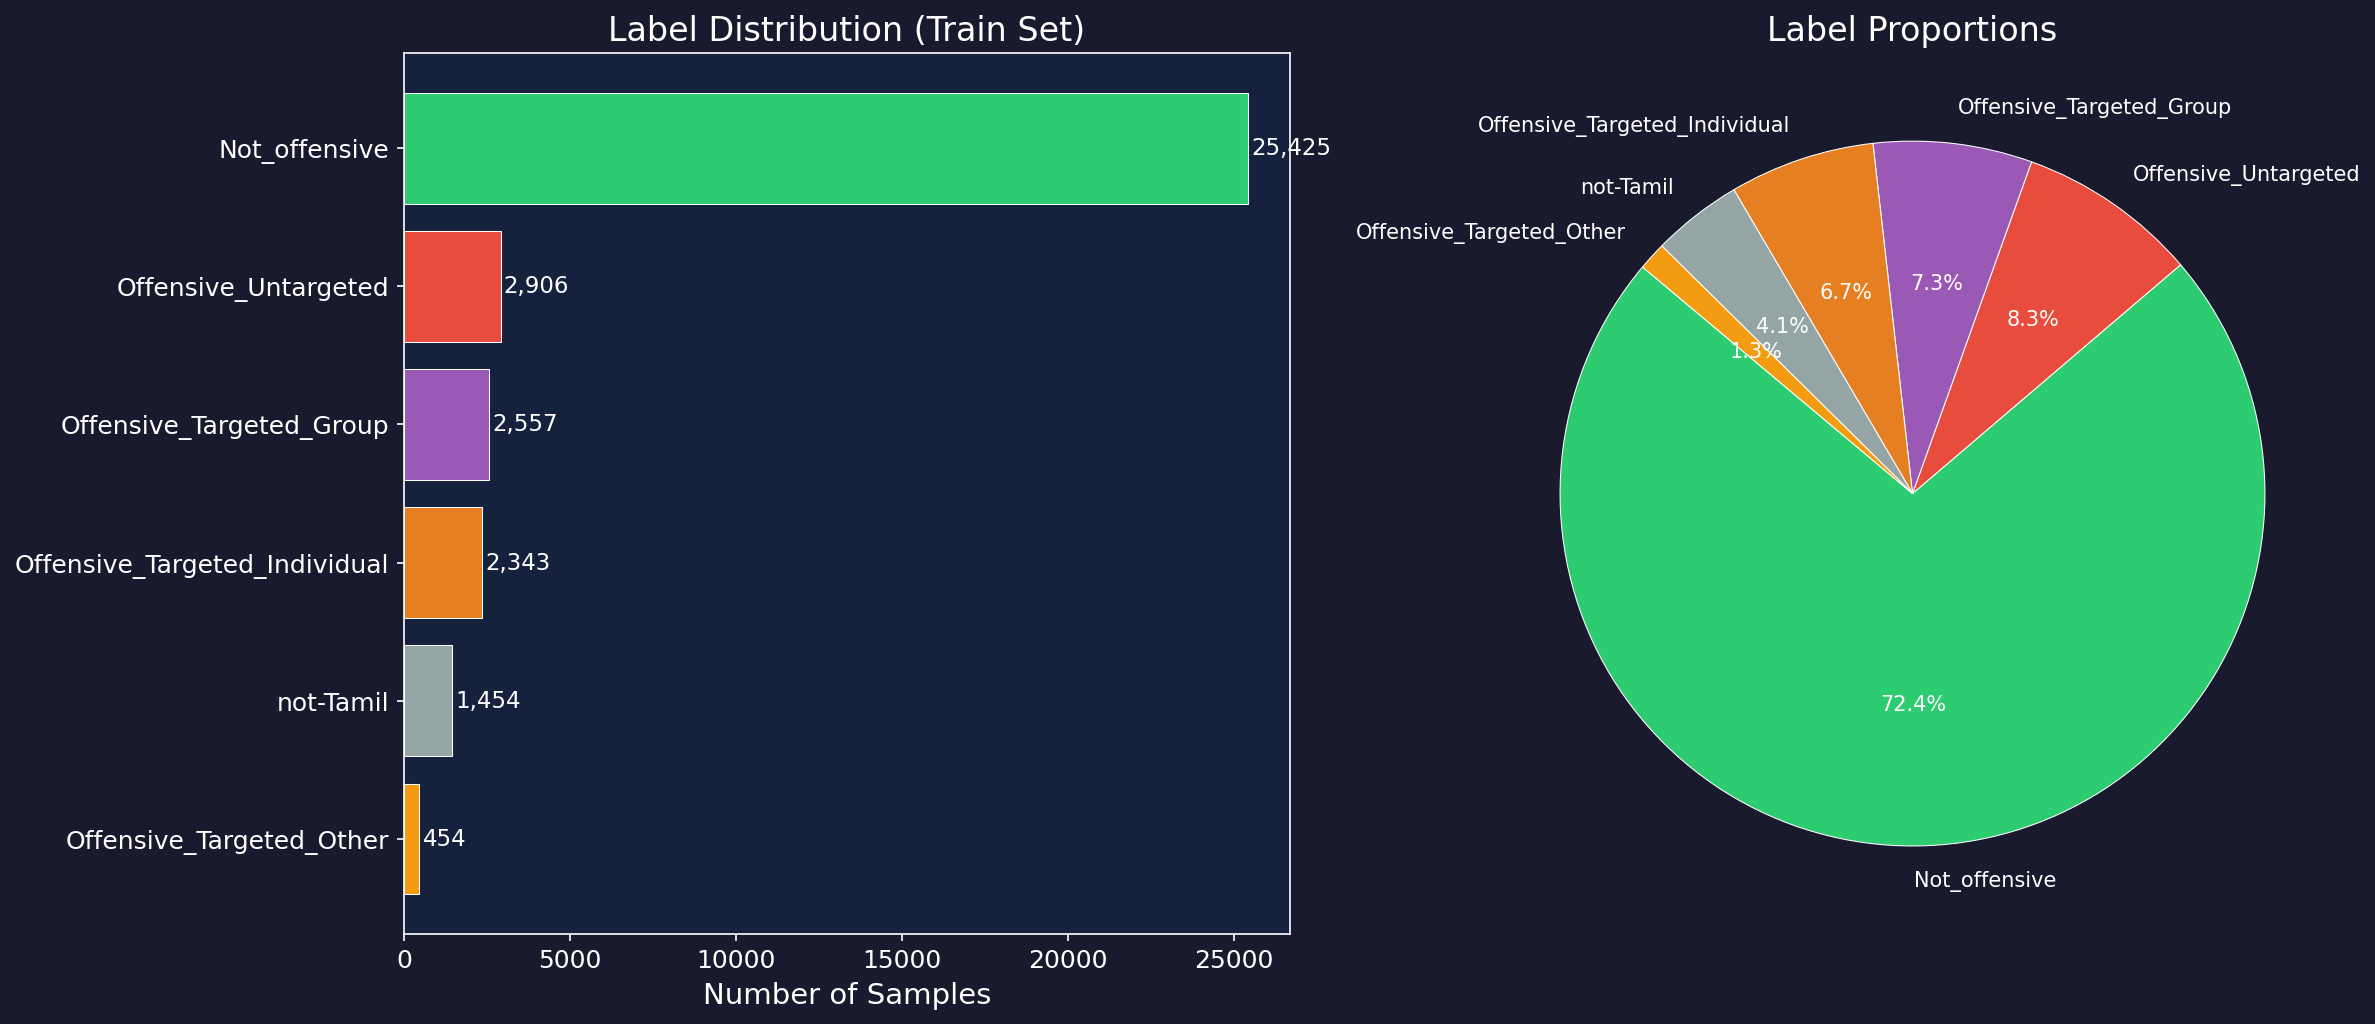
\includegraphics[width=0.95\textwidth]{figures/label_distribution.png}
\caption{Label distribution in the training set (left: horizontal bar chart; right: pie chart), illustrating the severe class imbalance. The \texttt{Not\_offensive} class dominates with 72.4\% of samples, while minority offensive sub-categories each represent less than 9\% of the data.}
\label{fig:label_dist}
\end{figure}

\FloatBarrier

\subsection{Script Analysis}

A distinctive feature of Tamil social media text is its script diversity. Our exploratory analysis reveals that the dataset contains content in three distinct script categories, as detailed in Table~\ref{tab:script_dist} and visualised in Figure~\ref{fig:script_dist}.

\begin{table}[!htbp]
\centering
\caption{Script type distribution in the training set. Latin-script (Tanglish) content dominates, reflecting the prevalence of transliterated Tamil on social media.}
\label{tab:script_dist}
\begin{tabular}{l r r}
\toprule
\textbf{Script Type} & \textbf{Count} & \textbf{Percentage (\%)} \\
\midrule
Latin (Tanglish/English) & 28,519 & 81.2 \\
Tamil Unicode            & 6,171  & 17.6 \\
Mixed (Code-Switched)    & 393    & 1.1  \\
Other                    & 56     & 0.2  \\
\bottomrule
\end{tabular}
\end{table}

\vspace{1em}

The overwhelming dominance of Latin-script content (81.2\%) is a striking finding that underscores a fundamental reality of Tamil social media: the majority of Tamil-speaking internet users prefer to type in Latin script (Tanglish) rather than Tamil Unicode, likely due to the ease of typing on standard QWERTY keyboards. This has significant implications for model selection, as models with stronger Latin-script handling may have an inherent advantage on this dataset.

\begin{figure}[!htbp]
\centering
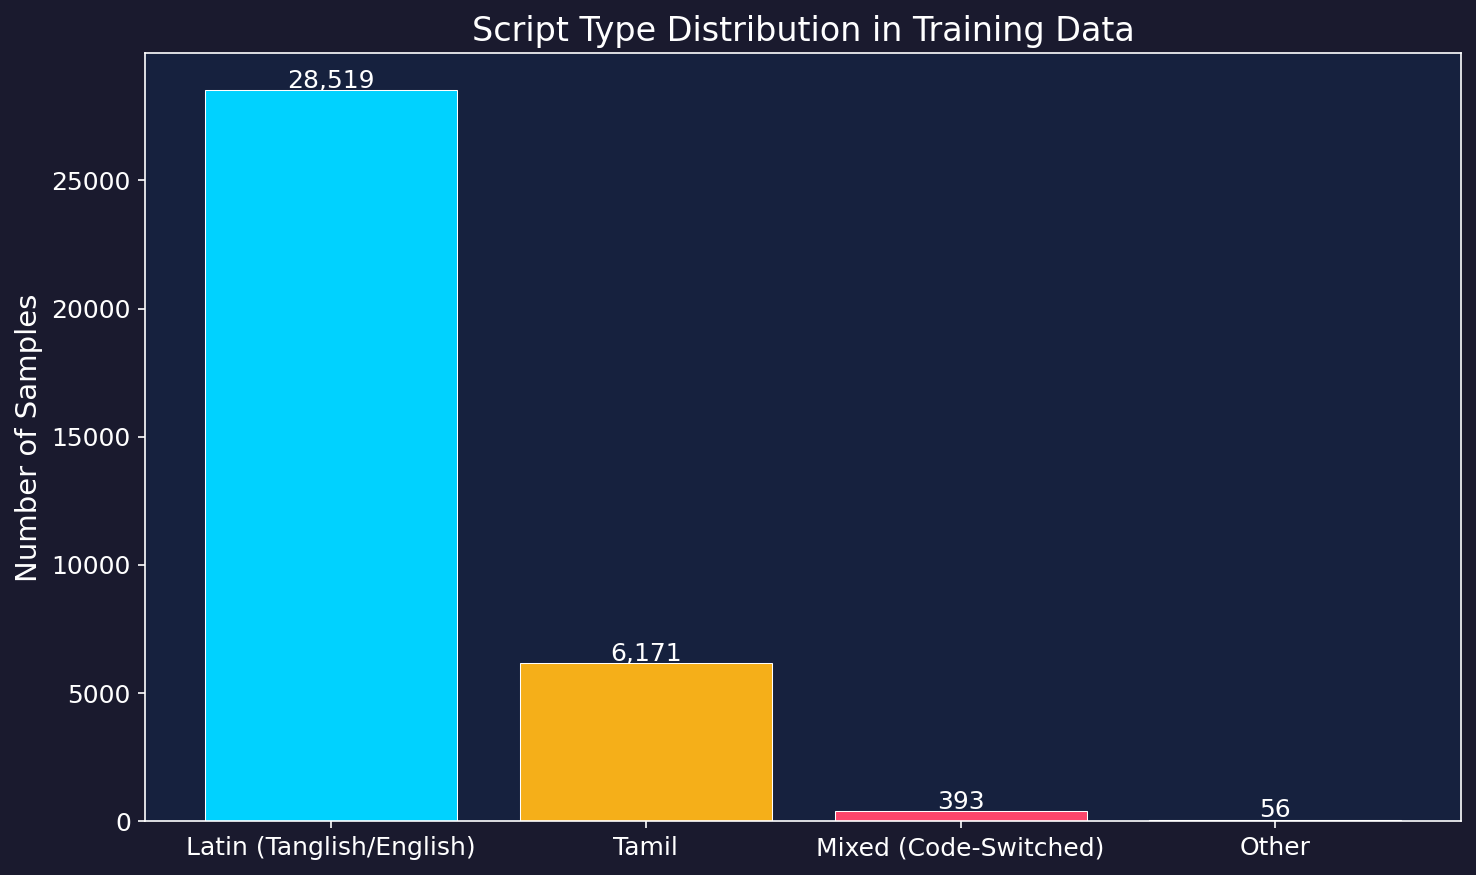
\includegraphics[width=0.7\textwidth]{figures/script_distribution.png}
\caption{Script type distribution in the training data, showing the dominance of Latin-script (Tanglish) content.}
\label{fig:script_dist}
\end{figure}

\FloatBarrier

\subsection{Text Length Characteristics}

Understanding the length distribution of social media comments is important for setting appropriate sequence length hyperparameters during model fine-tuning. Figure~\ref{fig:text_length} presents the character length and word count distributions across all six label categories.

\begin{figure}[!htbp]
\centering
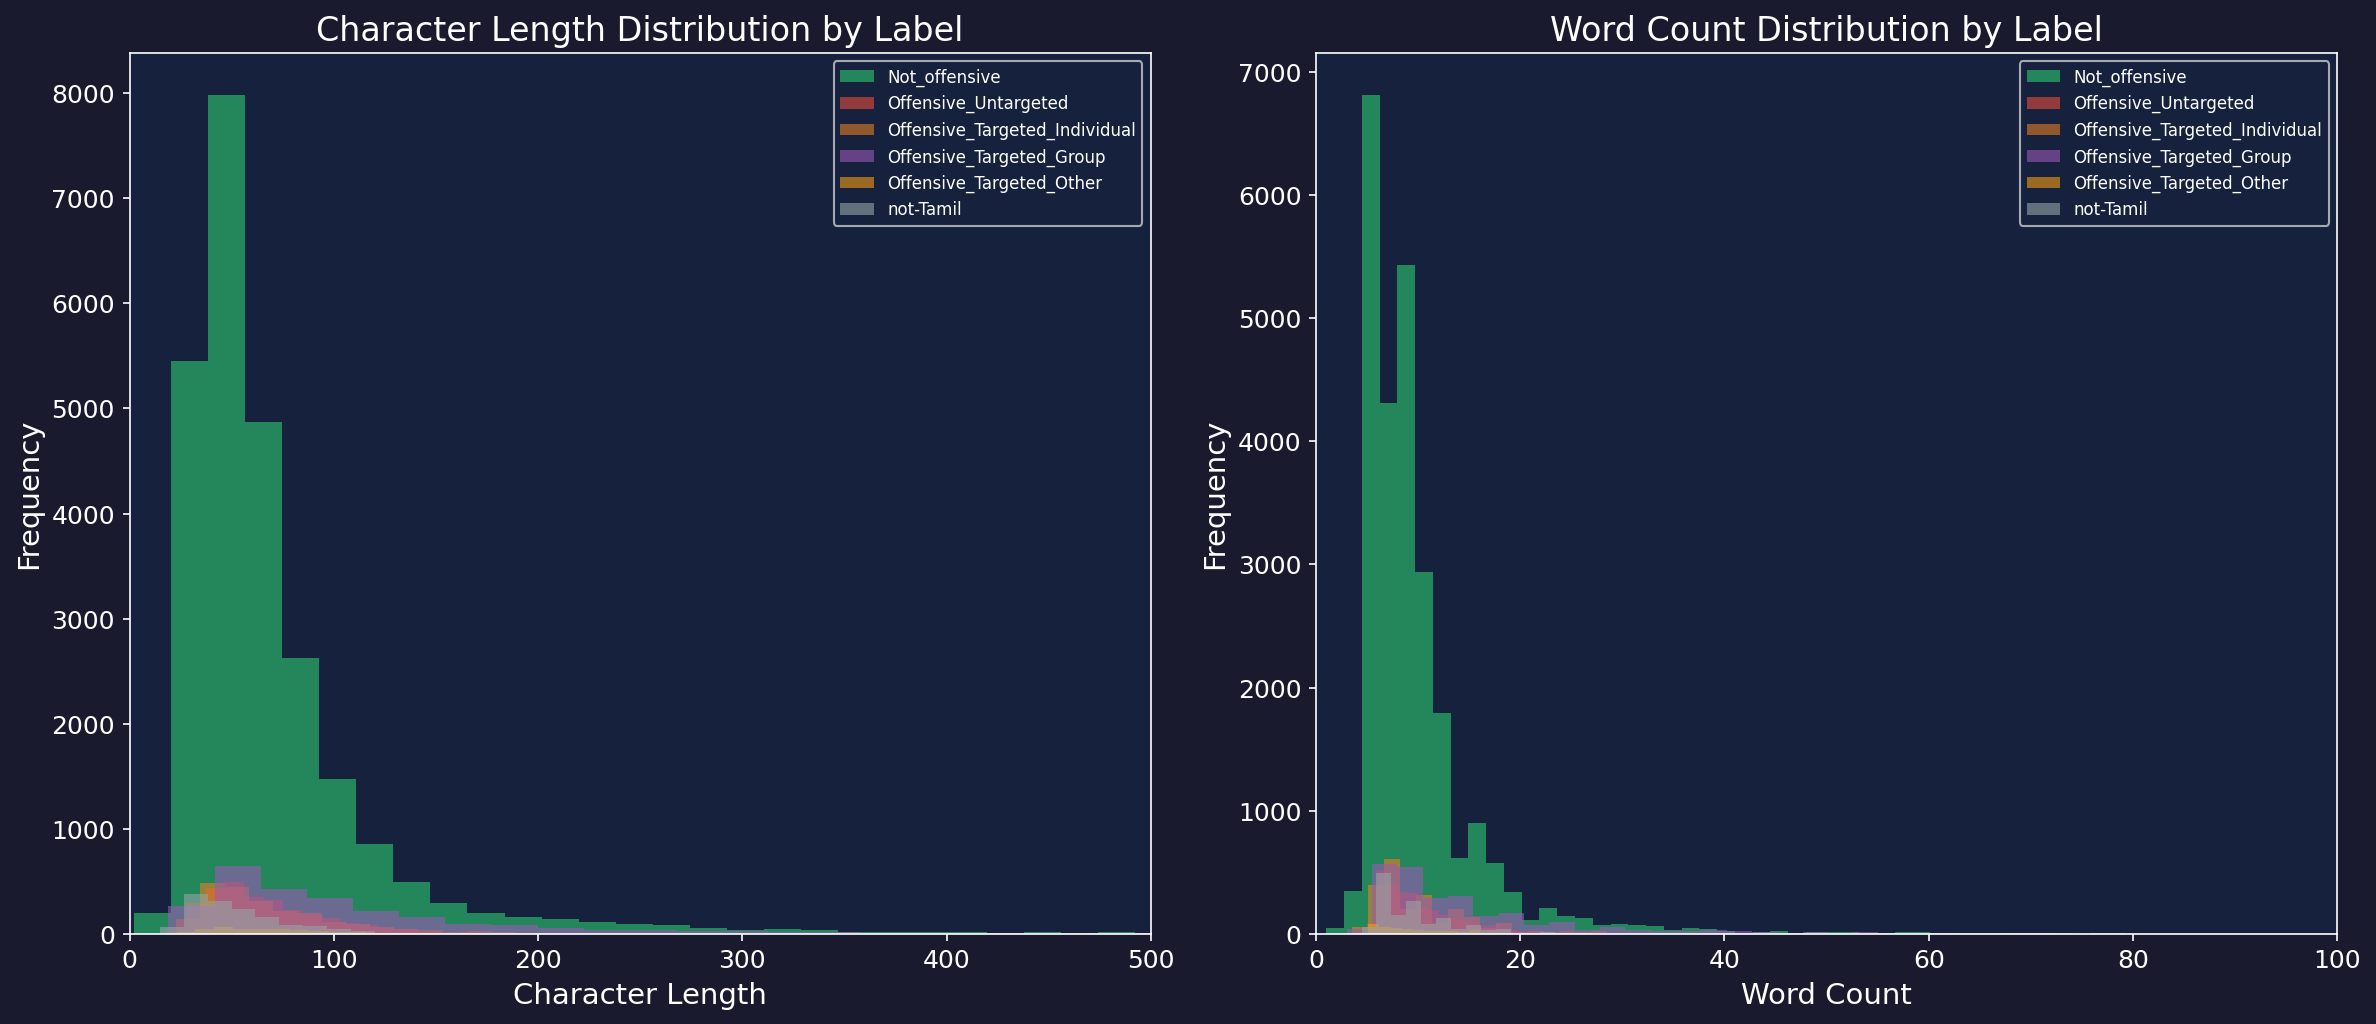
\includegraphics[width=0.95\textwidth]{figures/text_length_distribution.png}
\caption{Character length and word count distributions by label category. Most comments are short (fewer than 200 characters / 40 words), with offensive comments tending to be slightly longer than non-offensive ones.}
\label{fig:text_length}
\end{figure}

The majority of comments are relatively short, with a median character length of approximately 60 characters and a median word count of approximately 10 words. This is consistent with the informal, conversational nature of YouTube comments. The short average length justifies our choice of a maximum sequence length of 128 tokens for tokenisation, which accommodates the vast majority of samples without truncation.

\subsection{Script versus Label Interaction}

An important dimension of the dataset is the interaction between script type and offensive content distribution. Figure~\ref{fig:script_vs_label} presents a stacked bar chart showing the label distribution within each script category.

\begin{figure}[!htbp]
\centering
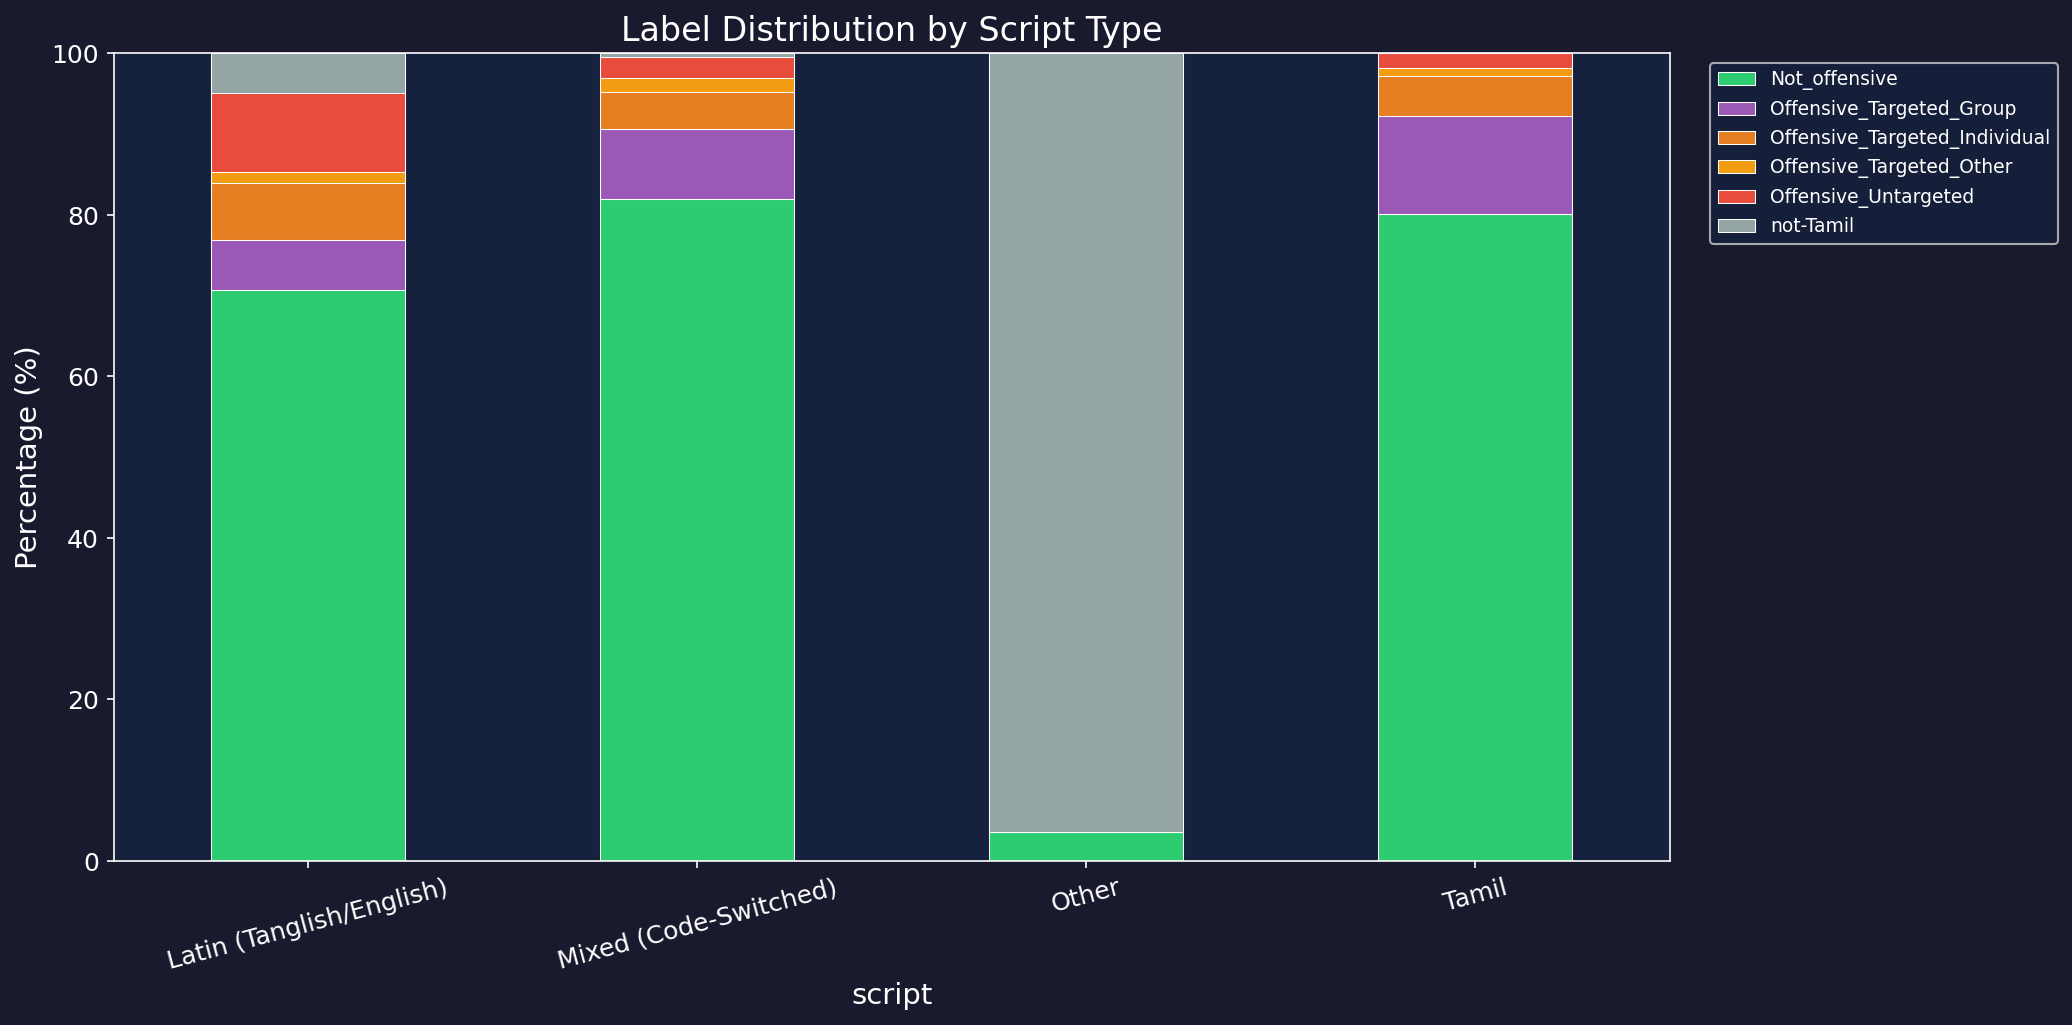
\includegraphics[width=0.85\textwidth]{figures/script_vs_label.png}
\caption{Label distribution by script type, showing that the proportion of offensive content varies across script categories.}
\label{fig:script_vs_label}
\end{figure}

\FloatBarrier

% ══════════════════════════════════════════════════════════════════════════════
\section{Methodology}
\label{sec:methodology}
% ══════════════════════════════════════════════════════════════════════════════

This section describes our complete pipeline for offensive language detection, from text preprocessing through model training to ensemble prediction and explainability analysis. Figure~\ref{fig:architecture} presents a high-level overview of the system architecture.

% ── System Architecture (TikZ) ────────────────────────────────────────────────

\begin{figure}[!htbp]
\centering
\resizebox{\textwidth}{!}{%
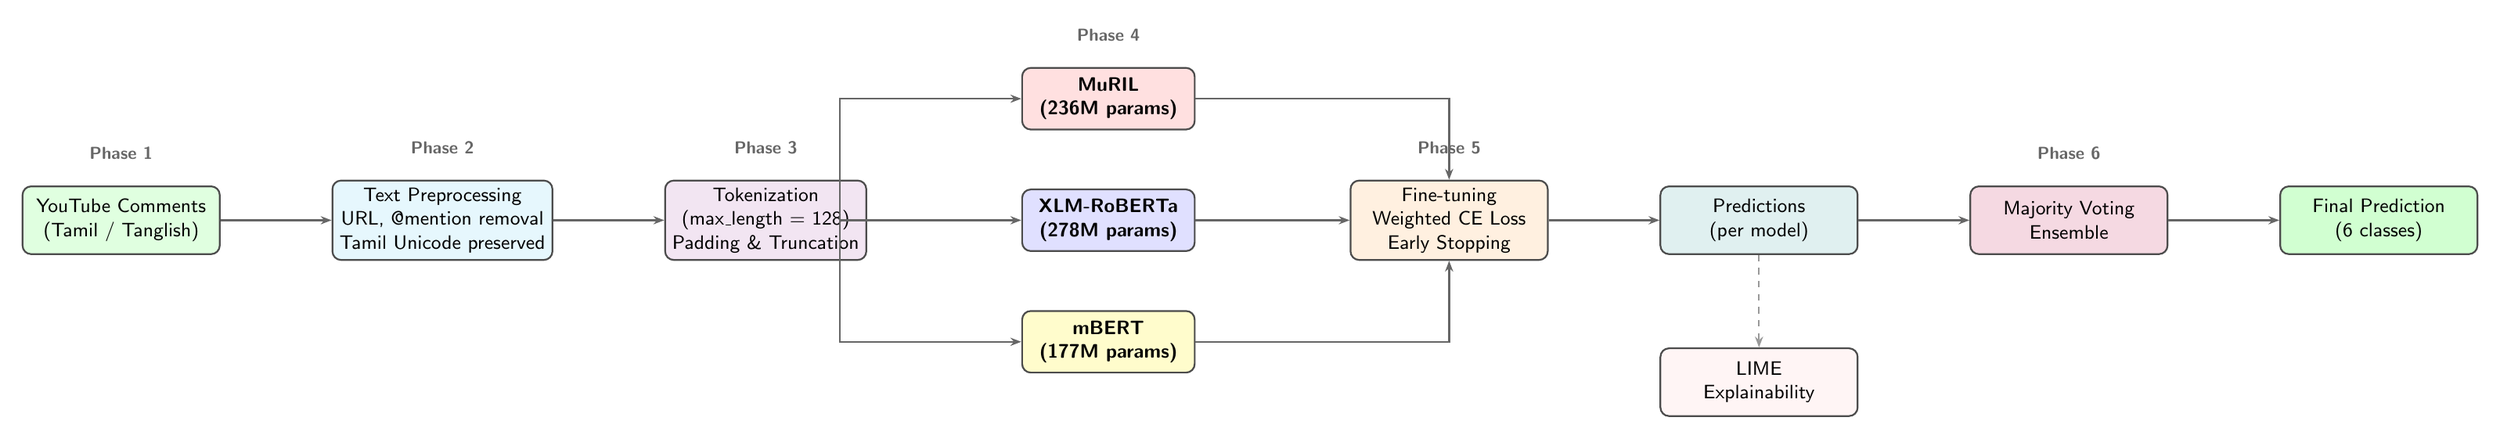
\begin{tikzpicture}[
    node distance=1.2cm and 1.8cm,
    box/.style={rectangle, draw=black!70, fill=#1, rounded corners=4pt, 
                minimum width=3.2cm, minimum height=1.1cm, align=center, 
                font=\small\sffamily, line width=0.8pt},
    box/.default={blue!8},
    modelbox/.style={rectangle, draw=black!70, fill=#1, rounded corners=4pt,
                     minimum width=2.8cm, minimum height=1.0cm, align=center,
                     font=\small\sffamily\bfseries, line width=0.8pt},
    modelbox/.default={orange!15},
    arrow/.style={-{Stealth[length=5pt]}, thick, draw=black!60},
    dashedarrow/.style={-{Stealth[length=5pt]}, thick, draw=black!40, dashed},
    grouplabel/.style={font=\footnotesize\sffamily\bfseries, text=black!60},
]

% Phase 1: Input
\node[box=green!12] (input) {YouTube Comments\\(Tamil / Tanglish)};

% Phase 2: Preprocessing
\node[box=cyan!10, right=of input] (preprocess) {Text Preprocessing\\URL, @mention removal\\Tamil Unicode preserved};

% Phase 3: Tokenization
\node[box=violet!10, right=of preprocess] (tokenize) {Tokenization\\(max\_length = 128)\\Padding \& Truncation};

% Phase 4: Three parallel models
\node[modelbox=red!12, above right=0.8cm and 2.5cm of tokenize] (muril) {MuRIL\\(236M params)};
\node[modelbox=blue!12, right=2.5cm of tokenize] (xlmr) {XLM-RoBERTa\\(278M params)};
\node[modelbox=yellow!20, below right=0.8cm and 2.5cm of tokenize] (mbert) {mBERT\\(177M params)};

% Phase 5: Training
\node[box=orange!12, right=2.5cm of xlmr] (train) {Fine-tuning\\Weighted CE Loss\\Early Stopping};

% Phase 6: Predictions
\node[box=teal!12, right=of train] (preds) {Predictions\\(per model)};

% Phase 7: Ensemble
\node[box=purple!15, right=of preds] (ensemble) {Majority Voting\\Ensemble};

% Phase 8: Output
\node[box=green!18, right=of ensemble] (output) {Final Prediction\\(6 classes)};

% Phase 9: LIME (below)
\node[box=pink!15, below=1.5cm of preds] (lime) {LIME\\Explainability};

% Arrows
\draw[arrow] (input) -- (preprocess);
\draw[arrow] (preprocess) -- (tokenize);

\draw[arrow] (tokenize) -- ++(1.2,0) |- (muril);
\draw[arrow] (tokenize) -- (xlmr);
\draw[arrow] (tokenize) -- ++(1.2,0) |- (mbert);

\draw[arrow] (muril) -| (train);
\draw[arrow] (xlmr) -- (train);
\draw[arrow] (mbert) -| (train);

\draw[arrow] (train) -- (preds);
\draw[arrow] (preds) -- (ensemble);
\draw[arrow] (ensemble) -- (output);

\draw[dashedarrow] (preds) -- (lime);

% Group labels
\node[grouplabel, above=0.3cm of input] {Phase 1};
\node[grouplabel, above=0.3cm of preprocess] {Phase 2};
\node[grouplabel, above=0.3cm of tokenize] {Phase 3};
\node[grouplabel, above=0.3cm of muril] {Phase 4};
\node[grouplabel, above=0.3cm of train] {Phase 5};
\node[grouplabel, above=0.3cm of ensemble] {Phase 6};

\end{tikzpicture}
}
\caption{System architecture overview. YouTube comments in Tamil and Tanglish undergo text preprocessing and tokenisation before being fed into three parallel multilingual transformer models (MuRIL, XLM-RoBERTa, mBERT). Each model is fine-tuned with weighted cross-entropy loss. Individual predictions are combined via majority-voting ensemble. LIME analysis is performed on the best individual model for explainability.}
\label{fig:architecture}
\end{figure}

\FloatBarrier

\subsection{Text Preprocessing}

The preprocessing pipeline is designed to normalise the noisy, informal text characteristic of YouTube comments while preserving linguistically meaningful features. The pipeline applies the following transformations in sequence:

\begin{enumerate}[leftmargin=2em]
    \item \textbf{URL removal:} All HTTP and HTTPS links are stripped from the text, as they carry no semantic information relevant to offensiveness classification.
    
    \item \textbf{Mention removal:} Twitter-style @mentions (which also appear in YouTube comments referencing other users) are removed to prevent the model from learning spurious associations between specific usernames and offensive content.
    
    \item \textbf{Hashtag normalisation:} The hash symbol (\#) is removed while preserving the hashtag text, as hashtags often contain meaningful content (e.g., \texttt{\#TamilCinema} $\rightarrow$ \texttt{TamilCinema}).
    
    \item \textbf{Character filtering:} Non-alphanumeric characters and special symbols are removed, with explicit preservation of the Tamil Unicode range (U+0B80--U+0BFF) to ensure that Tamil-script content is not damaged by the filtering process.
    
    \item \textbf{Case normalisation:} Latin characters are lowercased to reduce vocabulary size. Tamil script, being case-insensitive, is unaffected by this step.
    
    \item \textbf{Whitespace normalisation:} Multiple consecutive spaces are collapsed to a single space, and leading/trailing whitespace is stripped.
\end{enumerate}

Notably, we deliberately do not apply stemming or lemmatisation. Tamil morphology is agglutinative and highly complex, and existing Tamil stemmers are imperfect --- applying them risks destroying morphological cues that are important for offensiveness detection (e.g., verb suffixes indicating imperative mood, which can signal aggressive tone).

\subsection{Multilingual Transformer Models}

We evaluate three multilingual transformer models, each representing a different pre-training strategy. All three share the same underlying architecture --- the BERT encoder with 12 transformer layers, 768-dimensional hidden representations, and 12 self-attention heads --- but differ fundamentally in their pre-training data and objectives. Table~\ref{tab:model_specs} summarises their specifications.

\begin{table}[!htbp]
\centering
\caption{Specifications of the three multilingual transformer models used in this study. All models share the BERT-base architecture (12 layers, 768 hidden dimensions, 12 attention heads).}
\label{tab:model_specs}
\begin{tabular}{l c c p{5.5cm}}
\toprule
\textbf{Model} & \textbf{Parameters} & \textbf{Languages} & \textbf{Pre-training Data} \\
\midrule
MuRIL         & 236M & 17  & Indian web text, Wikipedia, CommonCrawl (Indian languages), plus transliterated and romanised text \\[0.5em]
XLM-RoBERTa   & 278M & 100 & CommonCrawl corpus (2.5 TB of text across 100 languages) \\[0.5em]
mBERT         & 177M & 104 & Wikipedia articles from 104 languages \\
\bottomrule
\end{tabular}
\end{table}

\vspace{1em}

\textbf{MuRIL} \citep{khanuja2021muril} is uniquely positioned for Indian-language NLP tasks. Unlike mBERT and XLM-RoBERTa, which are pre-trained on predominantly formal text (Wikipedia or web crawls), MuRIL explicitly includes transliterated and romanised Indian-language text in its pre-training data. This design choice directly addresses the prevalence of Tanglish and other romanised Indian-language text on social media. MuRIL supports 17 Indian languages, including Tamil, Hindi, Bengali, Telugu, Malayalam, and Kannada, and has demonstrated state-of-the-art performance on the IndicGLUE benchmark.

\textbf{XLM-RoBERTa} \citep{conneau2020xlmr} takes a different approach, opting for massive scale over language-specific curation. Trained on 2.5 terabytes of CommonCrawl data spanning 100 languages, XLM-RoBERTa benefits from a much larger and more diverse pre-training corpus than mBERT. It employs the RoBERTa training methodology --- dynamic masking, larger mini-batches, and longer training --- which has been shown to yield more robust representations. However, the ``curse of multilinguality'' \citep{conneau2020xlmr} means that capacity shared across 100 languages may leave less room for any single language, potentially disadvantaging low-resource languages like Tamil.

\textbf{mBERT} \citep{devlin2019bert} is the original multilingual BERT model, trained on the Wikipedia corpora of 104 languages using a shared 110,000-token WordPiece vocabulary. Despite being the oldest and smallest of the three models (177M parameters), mBERT has proven remarkably effective across a wide range of cross-lingual tasks. Its pre-training on Wikipedia, while smaller in scale than XLM-RoBERTa's CommonCrawl corpus, may confer advantages for languages with substantial Wikipedia presence.

For fine-tuning, we add a linear classification head on top of each model's \texttt{[CLS]} token representation, mapping the 768-dimensional contextual embedding to six class logits:

\begin{equation}
\hat{y} = \text{softmax}(W \cdot h_{\text{[CLS]}} + b)
\label{eq:classification}
\end{equation}

\noindent where $h_{\text{[CLS]}} \in \mathbb{R}^{768}$ is the final-layer representation of the \texttt{[CLS]} token, $W \in \mathbb{R}^{6 \times 768}$ and $b \in \mathbb{R}^{6}$ are learnable parameters, and $\hat{y} \in \mathbb{R}^{6}$ is the predicted probability distribution over the six classes.

\subsection{Class Imbalance Handling}

The severe class imbalance in the dataset (72.4\% majority class vs.\ 1.3\% rarest class) necessitates specialised loss functions. A standard cross-entropy loss would allow the model to achieve high accuracy by trivially predicting the majority class for every input. We employ inverse-frequency class weighting, which assigns higher loss penalties to misclassifications of underrepresented classes:

\begin{equation}
w_c = \frac{N}{C \times n_c}
\label{eq:class_weights}
\end{equation}

\noindent where $N$ is the total number of training samples, $C = 6$ is the number of classes, and $n_c$ is the number of samples in class $c$. The weighted cross-entropy loss is then:

\begin{equation}
\mathcal{L} = -\sum_{c=1}^{C} w_c \cdot y_c \cdot \log(\hat{y}_c)
\label{eq:weighted_ce}
\end{equation}

\noindent where $y_c$ is the one-hot encoded true label and $\hat{y}_c$ is the predicted probability for class $c$. The resulting class weights range from approximately 0.23 for \texttt{Not\_offensive} to approximately 12.9 for \texttt{Offensive\_Targeted\_Other}, forcing the model to pay disproportionately more attention to minority classes.

This approach is implemented through a custom \texttt{WeightedTrainer} class that overrides the default \texttt{Trainer.compute\_loss} method in the HuggingFace Transformers library. The key implementation detail is that labels are popped from the input dictionary before the forward pass, so the model produces unweighted logits, and the weighted loss is computed externally:

\begin{equation}
\text{loss} = \text{CrossEntropy}(\text{logits}, \text{labels}, \text{weight}=\mathbf{w})
\label{eq:implementation}
\end{equation}

\subsection{Training Configuration}

All three models are fine-tuned using identical hyperparameters to ensure a fair comparison. The hyperparameters, listed in Table~\ref{tab:hyperparams}, were selected based on established best practices for BERT fine-tuning \citep{devlin2019bert} and empirically validated on the validation set.

\begin{table}[!htbp]
\centering
\caption{Training hyperparameters used for all three models. These values represent established best practices for BERT fine-tuning on classification tasks.}
\label{tab:hyperparams}
\begin{tabular}{l l l}
\toprule
\textbf{Hyperparameter} & \textbf{Value} & \textbf{Rationale} \\
\midrule
Learning Rate          & $2 \times 10^{-5}$  & Standard for BERT fine-tuning \\
Effective Batch Size   & 32 (16 $\times$ 2)  & Via gradient accumulation \\
Max Sequence Length    & 128 tokens           & Sufficient for social media text \\
Training Epochs        & 5 (max)             & With early stopping \\
Early Stopping         & Patience = 2        & Based on validation F1-W \\
Weight Decay           & 0.01                & Light L2 regularisation \\
Warmup Ratio           & 0.1                 & Gradual LR increase \\
Optimizer              & AdamW               & Weight-decoupled Adam \\
Precision              & FP16 (mixed)        & Memory efficiency \\
Model Selection Metric & Weighted F1-Score   & Best for imbalanced data \\
\bottomrule
\end{tabular}
\end{table}

\vspace{1em}

A learning rate of $2 \times 10^{-5}$ is deliberately very small to avoid ``catastrophic forgetting'' --- the phenomenon where aggressive fine-tuning destroys the linguistic knowledge acquired during pre-training. The warmup ratio of 0.1 means that during the first 10\% of training steps, the learning rate linearly increases from zero to the target value, preventing large, destructive weight updates during the initial phase when gradients are noisy.

Early stopping with a patience of 2 epochs monitors the weighted F1-score on the validation set. If the validation metric does not improve for two consecutive epochs, training halts and the best checkpoint is restored. This prevents overfitting, which is particularly important given the relatively small size of the training set (35,138 samples) relative to the models' parameter counts (177--278 million).

Mixed-precision training (FP16) is employed to reduce GPU memory consumption by approximately 50\%, enabling the use of larger effective batch sizes on memory-constrained hardware. This is achieved through PyTorch's automatic mixed-precision (AMP) framework, which maintains a master copy of weights in FP32 for numerical stability while performing forward and backward passes in FP16.

\subsection{Ensemble Strategy}

To leverage the complementary strengths of the three models, we employ a majority-voting ensemble strategy. For each test sample, each of the three models independently predicts a class label, and the final prediction is the class that receives at least two out of three votes:

\begin{equation}
\hat{y}_{\text{ensemble}} = \text{mode}\left(\hat{y}_{\text{MuRIL}}, \hat{y}_{\text{XLM-R}}, \hat{y}_{\text{mBERT}}\right)
\label{eq:ensemble}
\end{equation}

Majority voting is an attractive ensemble strategy because it requires no additional training, introduces no hyperparameters, and is robust to individual model errors as long as the models' error patterns are sufficiently diverse. The intuition is that if two or more independently trained models agree on a prediction, it is more likely to be correct than a single model's prediction.

\subsection{Explainability with LIME}

To provide interpretability for model predictions, we employ LIME (Local Interpretable Model-agnostic Explanations) \citep{ribeiro2016lime}. For a given input text, LIME generates $N = 500$ perturbed versions by randomly removing words, obtains the model's prediction for each perturbed version, and fits a local linear model to learn the relationship between word presence/absence and the prediction. The resulting linear coefficients serve as word-level importance scores:

\begin{equation}
\text{explanation}(x) = \arg\min_{g \in G} \mathcal{L}(f, g, \pi_x) + \Omega(g)
\label{eq:lime}
\end{equation}

\noindent where $f$ is the model being explained, $g$ is the interpretable model (e.g., a linear model), $\pi_x$ is a proximity measure weighting perturbed instances by their distance to the original input $x$, and $\Omega(g)$ is a complexity penalty.

\FloatBarrier

% ══════════════════════════════════════════════════════════════════════════════
\section{Experimental Setup}
\label{sec:setup}
% ══════════════════════════════════════════════════════════════════════════════

\subsection{Hardware and Software Environment}

All model training was performed on a single NVIDIA Tesla T4 GPU (16 GB VRAM) via Google Colab Pro. The total training time for all three models was approximately 100 minutes. Evaluation and ensemble computation were performed on a local machine with an NVIDIA GeForce RTX 3050 (4 GB VRAM).

The software environment comprised Python 3.10, PyTorch 2.1, HuggingFace Transformers 4.35, HuggingFace Datasets 2.14, scikit-learn 1.3, and LIME 0.2. All experiments used a fixed random seed of 42 for reproducibility.

\subsection{Evaluation Metrics}

Given the severe class imbalance, we report multiple evaluation metrics to provide a comprehensive picture of model performance:

\begin{itemize}[leftmargin=2em]
    \item \textbf{Accuracy:} The fraction of correctly classified samples. While intuitive, accuracy is misleading for imbalanced datasets because a model predicting the majority class for every input achieves 72.4\% accuracy.
    
    \item \textbf{Weighted F1-Score (F1-W):} The harmonic mean of precision and recall, averaged across classes with weights proportional to class frequency. This is our \textit{primary evaluation metric}, as it accounts for class imbalance while giving more weight to more frequent classes.
    
    \item \textbf{Macro F1-Score (F1-M):} The unweighted average of per-class F1-scores. This metric treats all classes equally regardless of frequency, making it sensitive to performance on rare classes. It is our \textit{secondary metric} for assessing minority-class detection.
    
    \item \textbf{Weighted Precision (Prec-W) and Weighted Recall (Rec-W):} Provide additional granularity on the precision-recall trade-off.
    
    \item \textbf{Per-Class F1-Scores:} Individual F1-scores for each of the six classes, enabling fine-grained analysis of where models succeed and fail.
\end{itemize}

\subsection{Reproducibility Note}

All experiments reported in this paper use a single random seed (42). We acknowledge that results may vary with different random initialisations, and multi-seed experiments with confidence intervals are planned as future work. This is a common limitation in transformer fine-tuning studies, where the computational cost of multiple runs is non-trivial.

\FloatBarrier

% ══════════════════════════════════════════════════════════════════════════════
\section{Results and Analysis}
\label{sec:results}
% ══════════════════════════════════════════════════════════════════════════════

\subsection{Overall Performance}

Table~\ref{tab:overall_results} presents the overall performance of all three individual models and the majority-voting ensemble on the test set.

\begin{table}[!htbp]
\centering
\caption{Overall performance comparison on the test set (2,194 samples). The best individual result per metric is \underline{underlined}; the best overall result is in \textbf{bold}.}
\label{tab:overall_results}
\begin{tabular}{l c c c c c}
\toprule
\textbf{Model} & \textbf{Accuracy} & \textbf{F1-W} & \textbf{F1-M} & \textbf{Prec-W} & \textbf{Rec-W} \\
\midrule
MuRIL          & 0.7115 & 0.7310 & 0.4405 & 0.7637 & 0.7115 \\
XLM-RoBERTa    & 0.7019 & 0.7275 & 0.4743 & 0.7791 & 0.7019 \\
mBERT          & \underline{0.7288} & \underline{0.7505} & \underline{0.4972} & \underline{0.7840} & \underline{0.7288} \\
\midrule
\textbf{Ensemble} & \textbf{0.7502} & \textbf{0.7620} & 0.4947 & \textbf{0.7817} & \textbf{0.7502} \\
\bottomrule
\end{tabular}
\end{table}

\vspace{1em}

Several observations emerge from these results. First, \textbf{mBERT achieves the highest individual performance} across all metrics, with a weighted F1-score of 0.7505. This is a somewhat surprising result, given that mBERT is the oldest and smallest of the three models (177M parameters vs.\ 236M for MuRIL and 278M for XLM-RoBERTa). Second, \textbf{the ensemble improves over the best individual model} on weighted metrics (F1-W: 0.7620 vs.\ 0.7505, an improvement of +1.15\% absolute), confirming that the three models capture complementary aspects of the linguistic signal. Third, the ensemble's F1-Macro (0.4947) is slightly lower than mBERT's (0.4972), reflecting the well-known trade-off in majority voting: the ensemble tends to favour the majority class, improving weighted metrics at the cost of minority-class performance.

Figure~\ref{fig:model_comparison} provides a visual comparison of the evaluation metrics across all four systems.

\begin{figure}[!htbp]
\centering
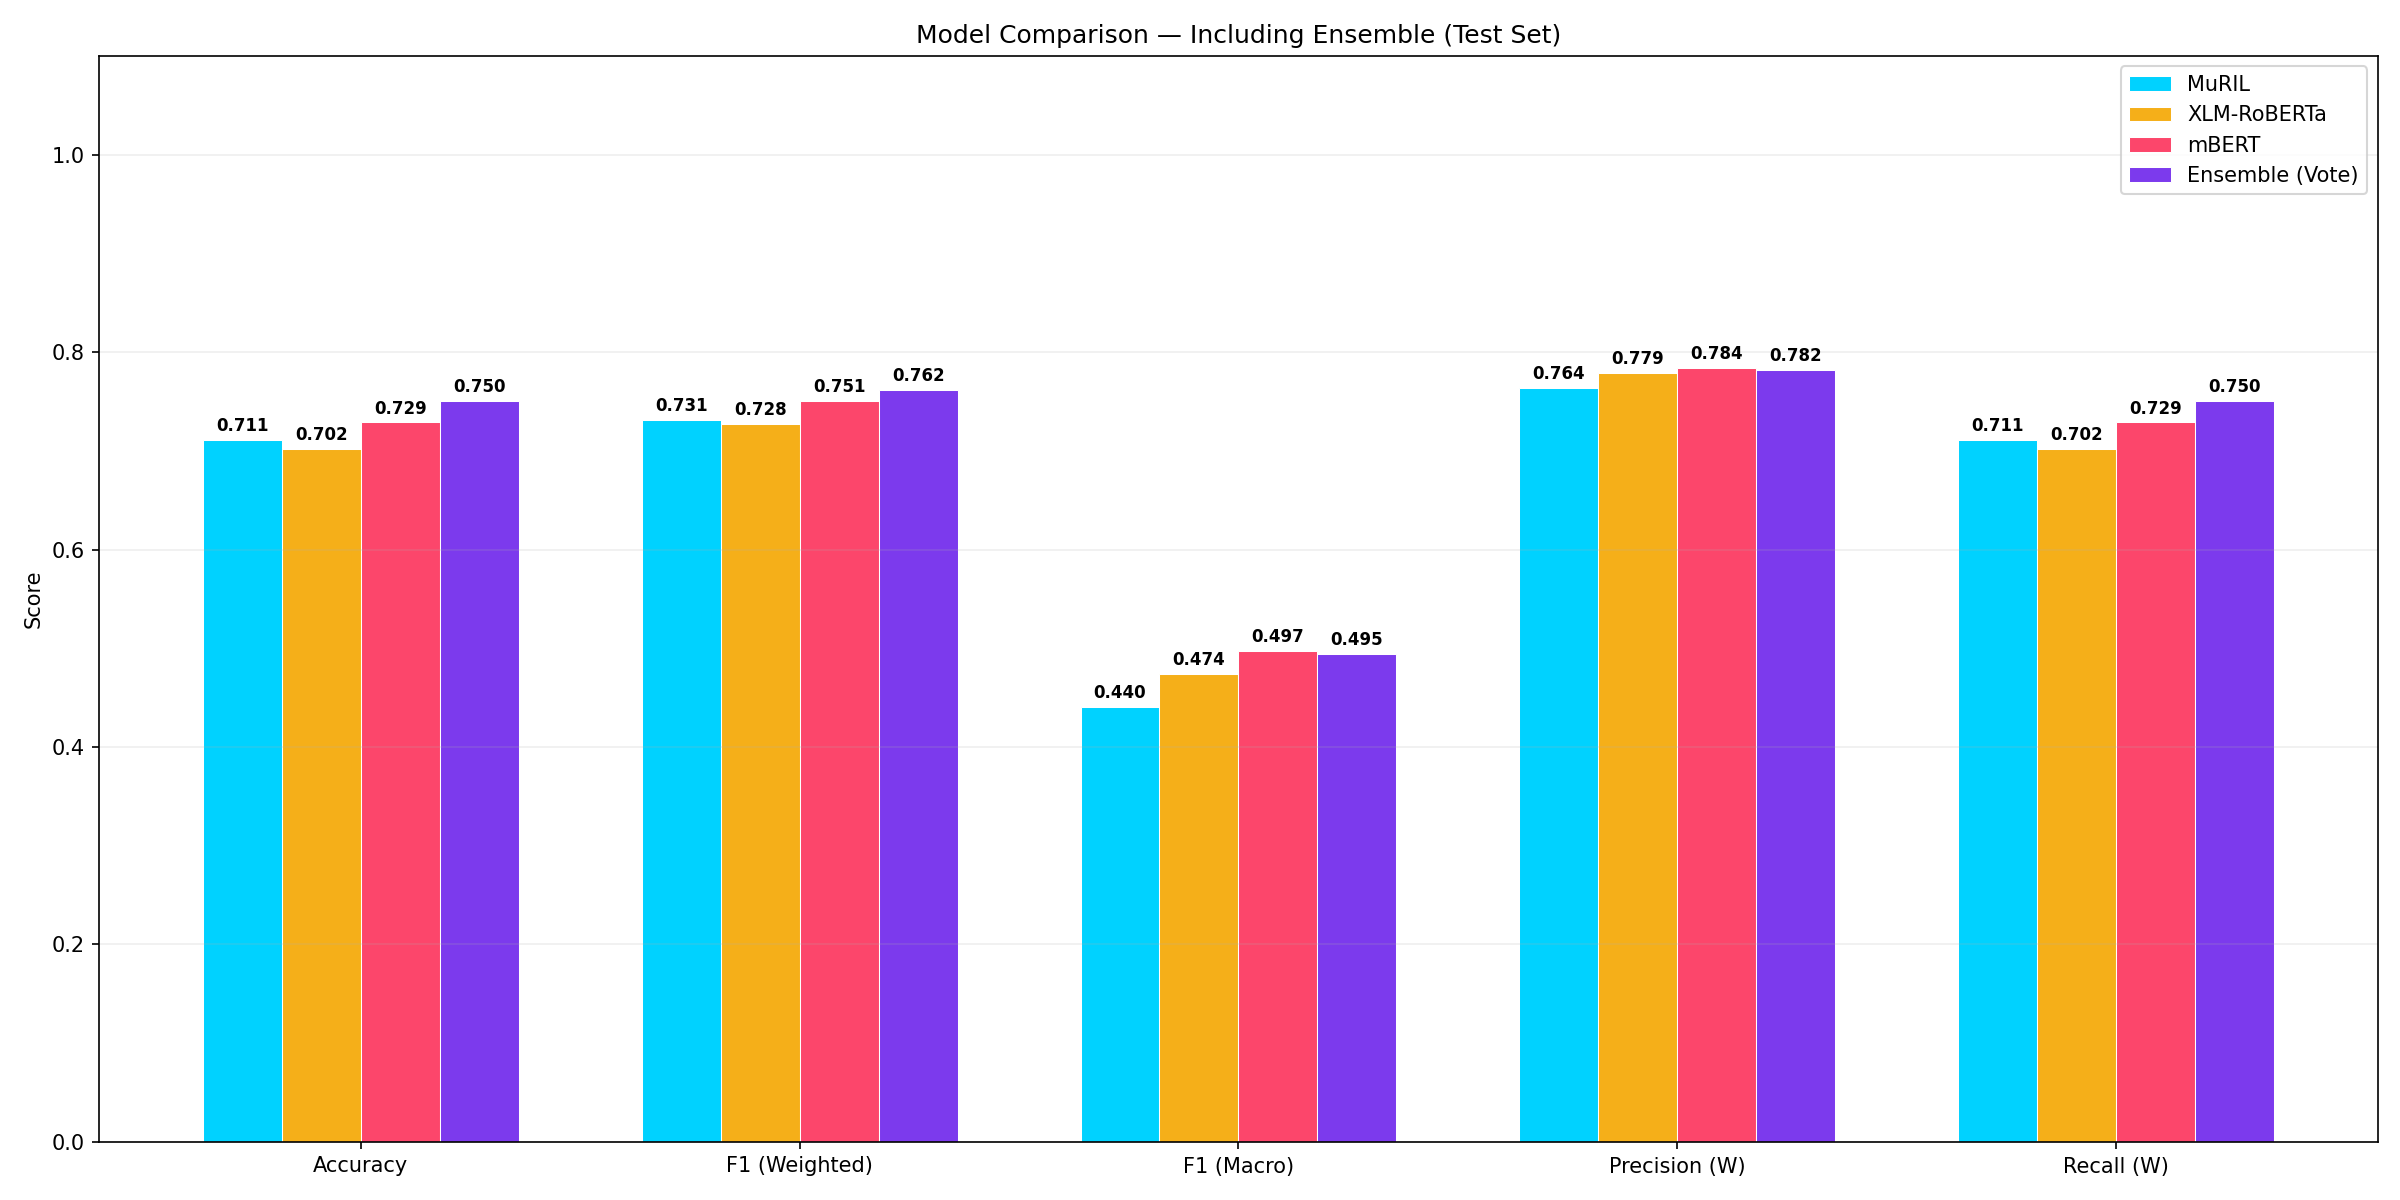
\includegraphics[width=0.85\textwidth]{figures/model_comparison_with_ensemble.png}
\caption{Bar chart comparing evaluation metrics (Accuracy, F1-Weighted, F1-Macro, Precision-Weighted, Recall-Weighted) across the three individual models and the ensemble.}
\label{fig:model_comparison}
\end{figure}

\FloatBarrier

\subsection{Contextualisation with Shared Task Results}

To provide context for our results, Table~\ref{tab:shared_task} presents approximate scores from the DravidianLangTech-2021 shared task. We emphasise that \textit{direct comparison is not valid} because we use a different test split.

\begin{table}[!htbp]
\centering
\caption{Contextual comparison with DravidianLangTech-2021 shared task results. Direct comparison is not valid due to different test sets.}
\label{tab:shared_task}
\begin{tabular}{l c l}
\toprule
\textbf{System} & \textbf{F1-W} & \textbf{Test Set} \\
\midrule
hate-alert (1st place) \citep{chakravarthi2021dravidian} & 0.78$^\dagger$ & Official \\
Top-5 range \citep{chakravarthi2021dravidian} & 0.75--0.78$^\dagger$ & Official \\
Median participant \citep{chakravarthi2021dravidian} & $\approx$0.70$^\dagger$ & Official \\
\midrule
mBERT (ours) & 0.7505 & Custom split \\
Ensemble (ours) & 0.7620 & Custom split \\
\bottomrule
\multicolumn{3}{l}{\footnotesize $^\dagger$ Tested on the official shared task test set; not directly comparable.}
\end{tabular}
\end{table}

\vspace{1em}

Our ensemble's weighted F1-score of 0.7620 falls within the competitive range of the shared task's top-performing systems, suggesting that our approach is broadly competitive despite using only standard fine-tuning without advanced techniques such as data augmentation or multi-task learning.

\subsection{Per-Class Performance Analysis}

Table~\ref{tab:perclass_f1} presents per-class F1-scores for all four systems, providing a more granular view of model strengths and weaknesses.

\begin{table}[!htbp]
\centering
\caption{Per-class F1-scores on the test set. The best result per class is in \textbf{bold}. The \texttt{Offensive\_Targeted\_Other} class remains largely undetectable across all approaches.}
\label{tab:perclass_f1}
\begin{tabular}{l c c c c}
\toprule
\textbf{Class} & \textbf{MuRIL} & \textbf{XLM-R} & \textbf{mBERT} & \textbf{Ensemble} \\
\midrule
Not\_offensive              & 0.863 & 0.835 & 0.863 & \textbf{0.876} \\
Offensive\_Untargeted       & 0.383 & 0.411 & 0.405 & \textbf{0.430} \\
Off.\_Targeted\_Individual  & 0.230 & 0.421 & \textbf{0.445} & 0.425 \\
Off.\_Targeted\_Group       & 0.321 & 0.362 & 0.360 & \textbf{0.377} \\
Off.\_Targeted\_Other       & 0.000 & 0.000 & \textbf{0.082} & 0.000 \\
not-Tamil                   & 0.846 & 0.817 & 0.828 & \textbf{0.860} \\
\bottomrule
\end{tabular}
\end{table}

\vspace{1em}

The per-class results reveal several important patterns:

\begin{enumerate}[leftmargin=2em]
    \item \textbf{Strong majority-class detection:} All models achieve F1 $>$ 0.83 on the \texttt{Not\_offensive} class, with the ensemble reaching 0.876. This high performance on the majority class drives the overall weighted F1-scores.
    
    \item \textbf{Reliable language identification:} The \texttt{not-Tamil} class is detected with F1 $>$ 0.81 across all models, demonstrating that the models can effectively distinguish non-Tamil content even without explicit language identification features.
    
    \item \textbf{Moderate offensive sub-type detection:} The intermediate offensive classes (\texttt{Untargeted}, \texttt{Targeted\_Individual}, \texttt{Targeted\_Group}) achieve F1-scores in the 0.23--0.45 range, reflecting the inherent difficulty of fine-grained offensive language classification.
    
    \item \textbf{Near-zero performance on the rarest class:} The \texttt{Offensive\_Targeted\_Other} class, with only approximately 30 test samples (1.3\% of training data), achieves F1 of 0.000 for MuRIL, XLM-RoBERTa, and the ensemble, with only mBERT managing a minimal F1 of 0.082. This class is effectively undetectable with current approaches, highlighting the fundamental limitation of training on severely underrepresented categories.
    
    \item \textbf{Ensemble benefits:} The ensemble achieves the best F1 on 4 out of 6 classes, confirming that model diversity yields complementary error patterns.
\end{enumerate}

\subsection{Performance by Script Type}

One of the most revealing analyses in this study is the breakdown of model performance by script type, presented in Table~\ref{tab:script_performance}.

\begin{table}[!htbp]
\centering
\caption{Weighted F1-score by script type on the test set. MuRIL excels on pure Tamil Unicode text, while mBERT dominates on Latin/Tanglish text.}
\label{tab:script_performance}
\begin{tabular}{l r c c c c}
\toprule
\textbf{Script} & \textbf{N} & \textbf{MuRIL} & \textbf{XLM-R} & \textbf{mBERT} & \textbf{Ensemble} \\
\midrule
Latin (Tanglish) & 1,762 & 0.719 & 0.717 & \underline{0.749} & \textbf{0.756} \\
Tamil Unicode    & 416   & \underline{0.771} & 0.758 & 0.747 & \textbf{0.775} \\
Mixed            & 12    & 0.741 & 0.782 & \underline{0.796} & \textbf{0.845} \\
\bottomrule
\end{tabular}
\end{table}

\vspace{1em}

This analysis reveals a key finding: \textbf{MuRIL is the best individual model on pure Tamil Unicode text} (F1-W: 0.771), outperforming both mBERT (0.747) and XLM-RoBERTa (0.758). This confirms that MuRIL's Indian-language-specific pre-training does provide genuine advantages for native-script Tamil content. However, \textbf{mBERT dominates on Latin/Tanglish text} (0.749 vs.\ MuRIL's 0.719), and since Latin-script content constitutes 80\% of the test set, mBERT's Tanglish advantage drives its overall superiority. The ensemble achieves the best performance across all three script categories.

\subsection{Confusion Matrix Analysis}

Figures~\ref{fig:cm_mbert} and \ref{fig:cm_ensemble} present the confusion matrices for mBERT and the ensemble, respectively. Additional confusion matrices for MuRIL and XLM-RoBERTa are provided in Figures~\ref{fig:cm_muril} and \ref{fig:cm_xlmr}.

\begin{figure}[!htbp]
\centering
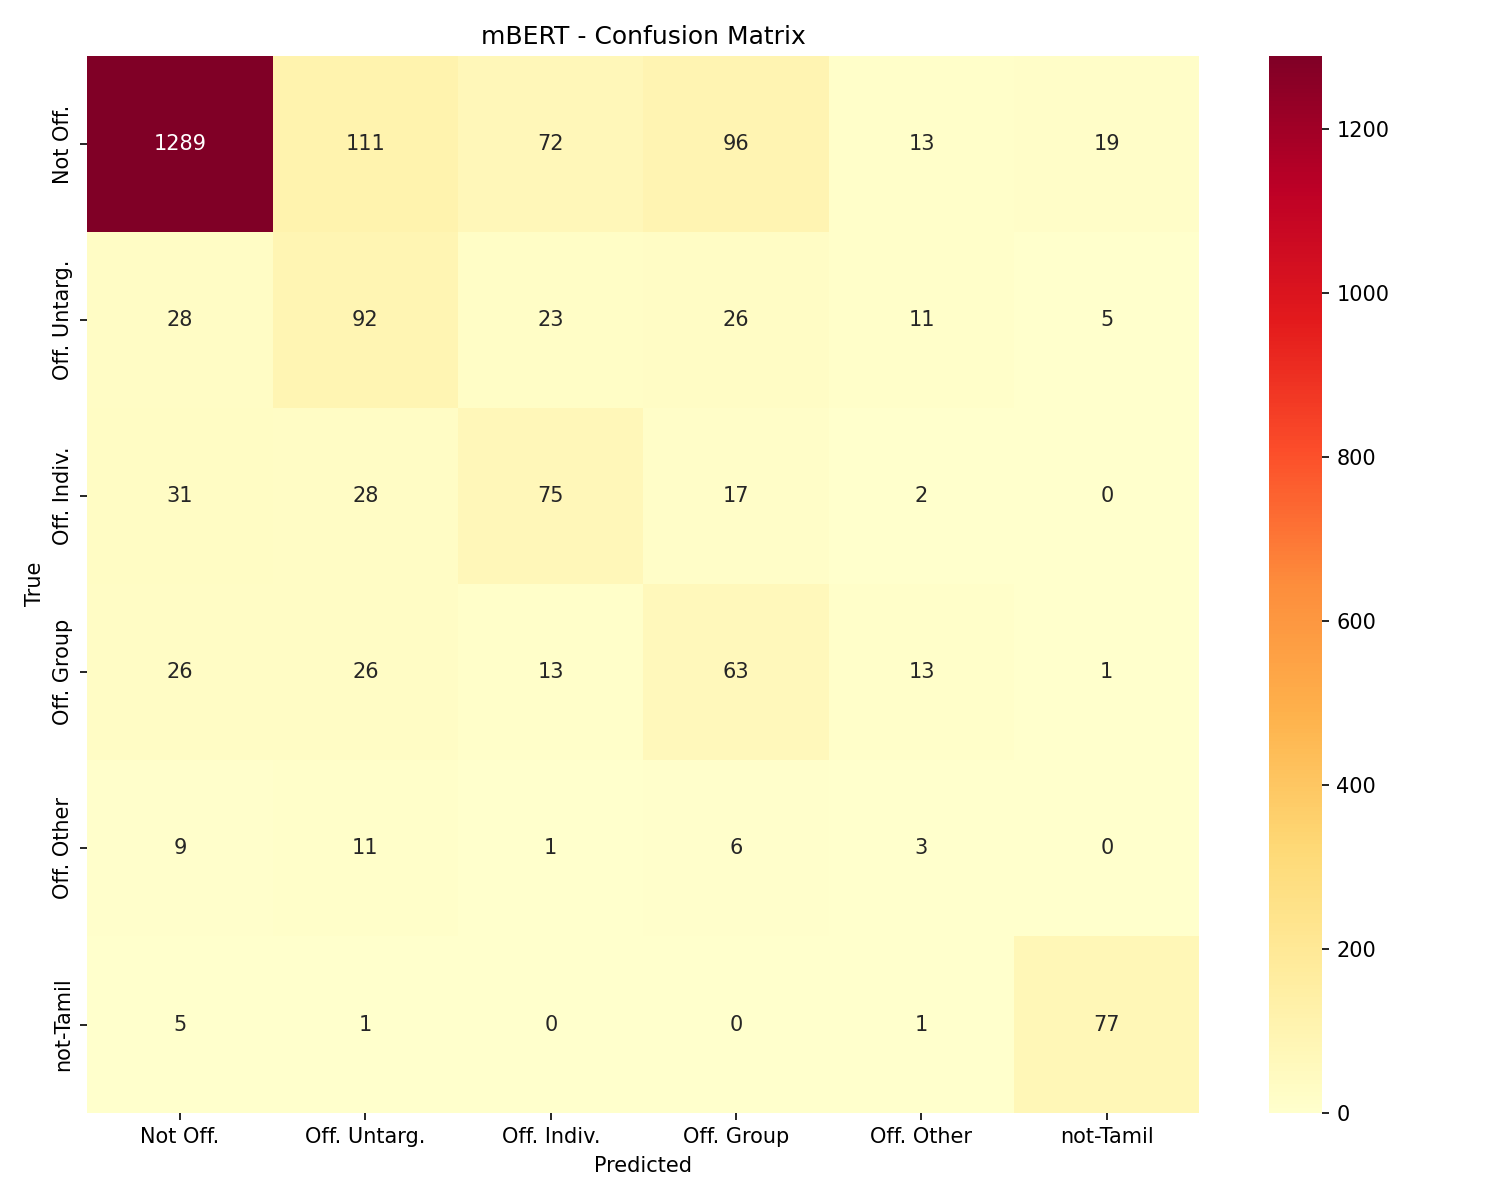
\includegraphics[width=0.75\textwidth]{figures/mbert_confusion_matrix.png}
\caption{Confusion matrix for mBERT on the test set. The dominant error pattern is the misclassification of offensive content as \texttt{Not\_offensive} (false negatives), visible in the first column.}
\label{fig:cm_mbert}
\end{figure}

\begin{figure}[!htbp]
\centering
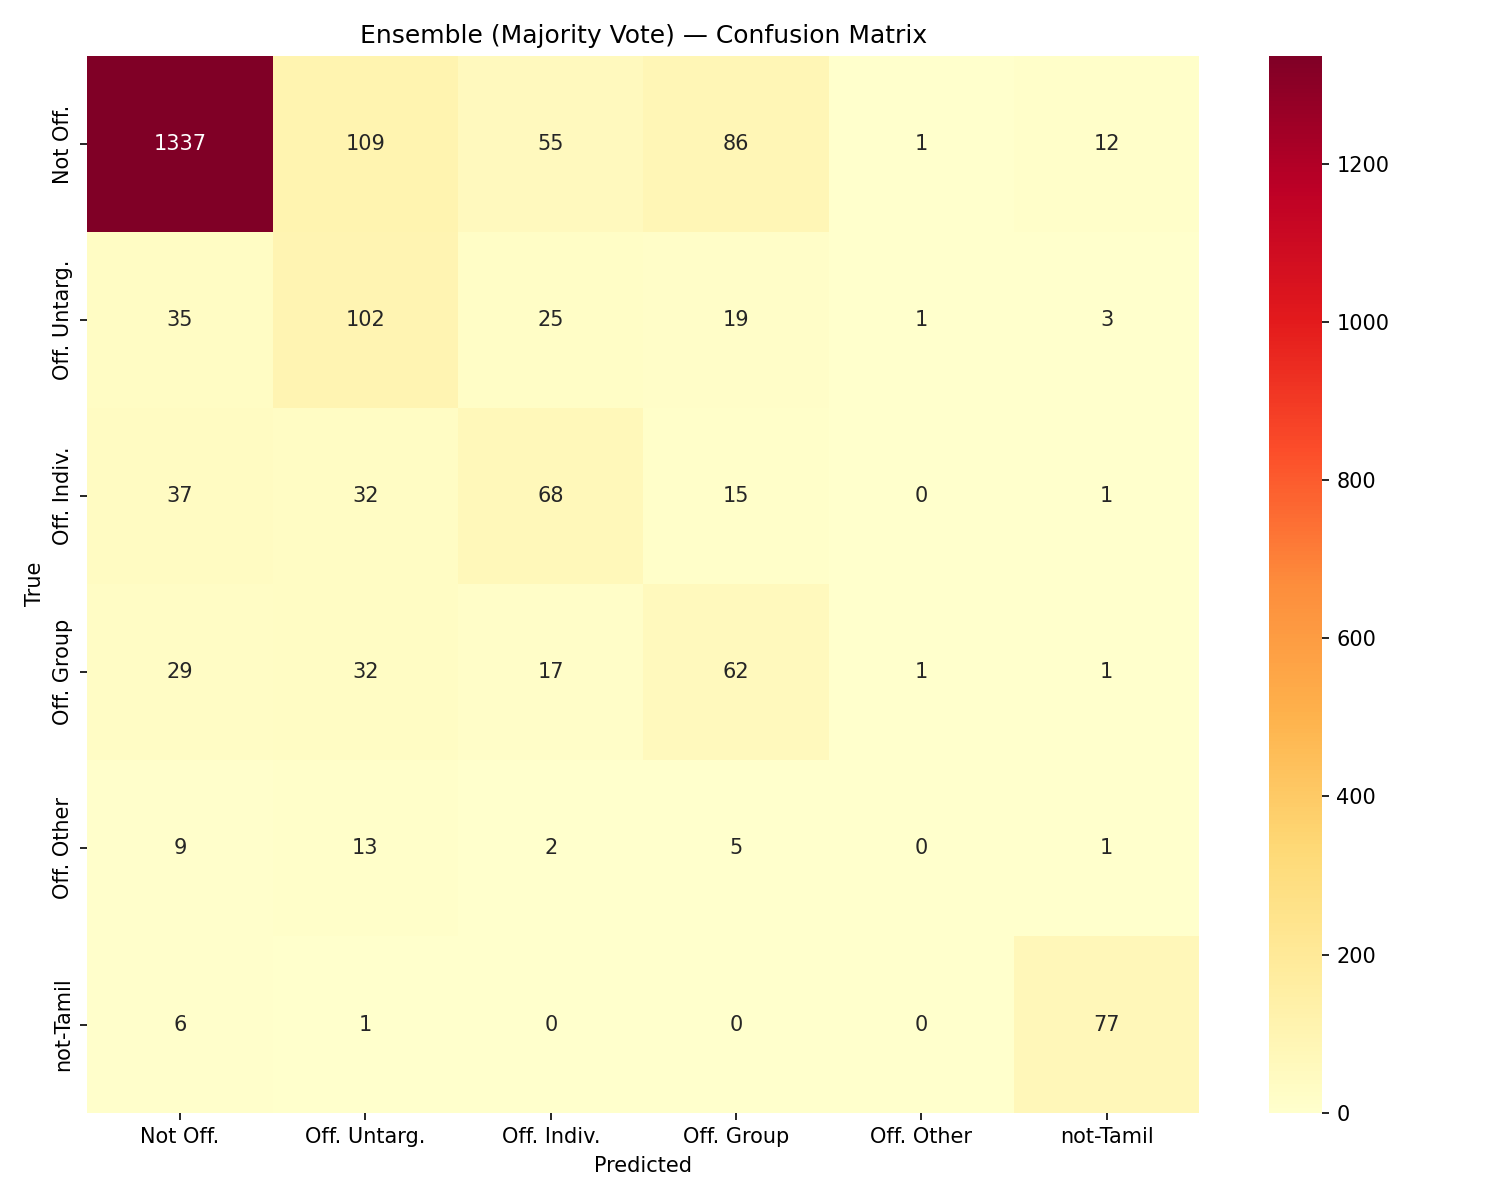
\includegraphics[width=0.75\textwidth]{figures/ensemble_confusion_matrix.png}
\caption{Confusion matrix for the majority-voting ensemble on the test set. The ensemble reduces errors in the majority class but inherits the near-zero detection of \texttt{Offensive\_Targeted\_Other}.}
\label{fig:cm_ensemble}
\end{figure}

\begin{figure}[!htbp]
\centering
\begin{subfigure}[b]{0.48\textwidth}
    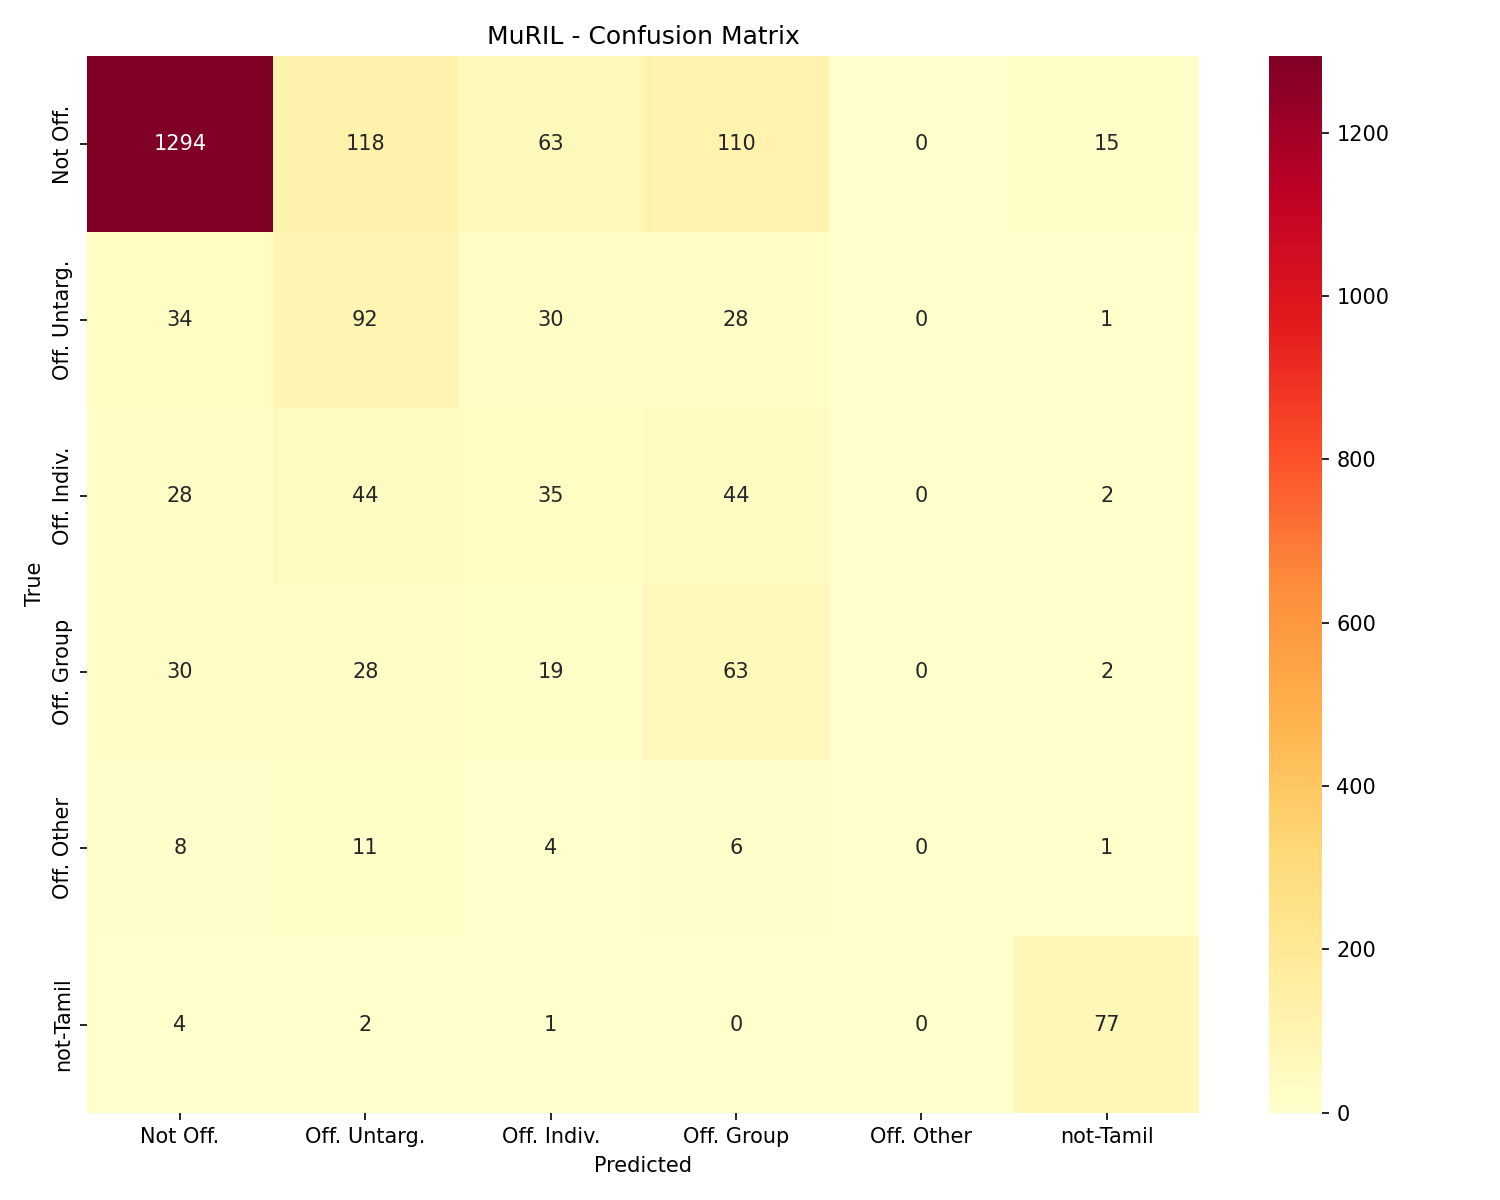
\includegraphics[width=\textwidth]{figures/muril_confusion_matrix.png}
    \caption{MuRIL}
    \label{fig:cm_muril}
\end{subfigure}
\hfill
\begin{subfigure}[b]{0.48\textwidth}
    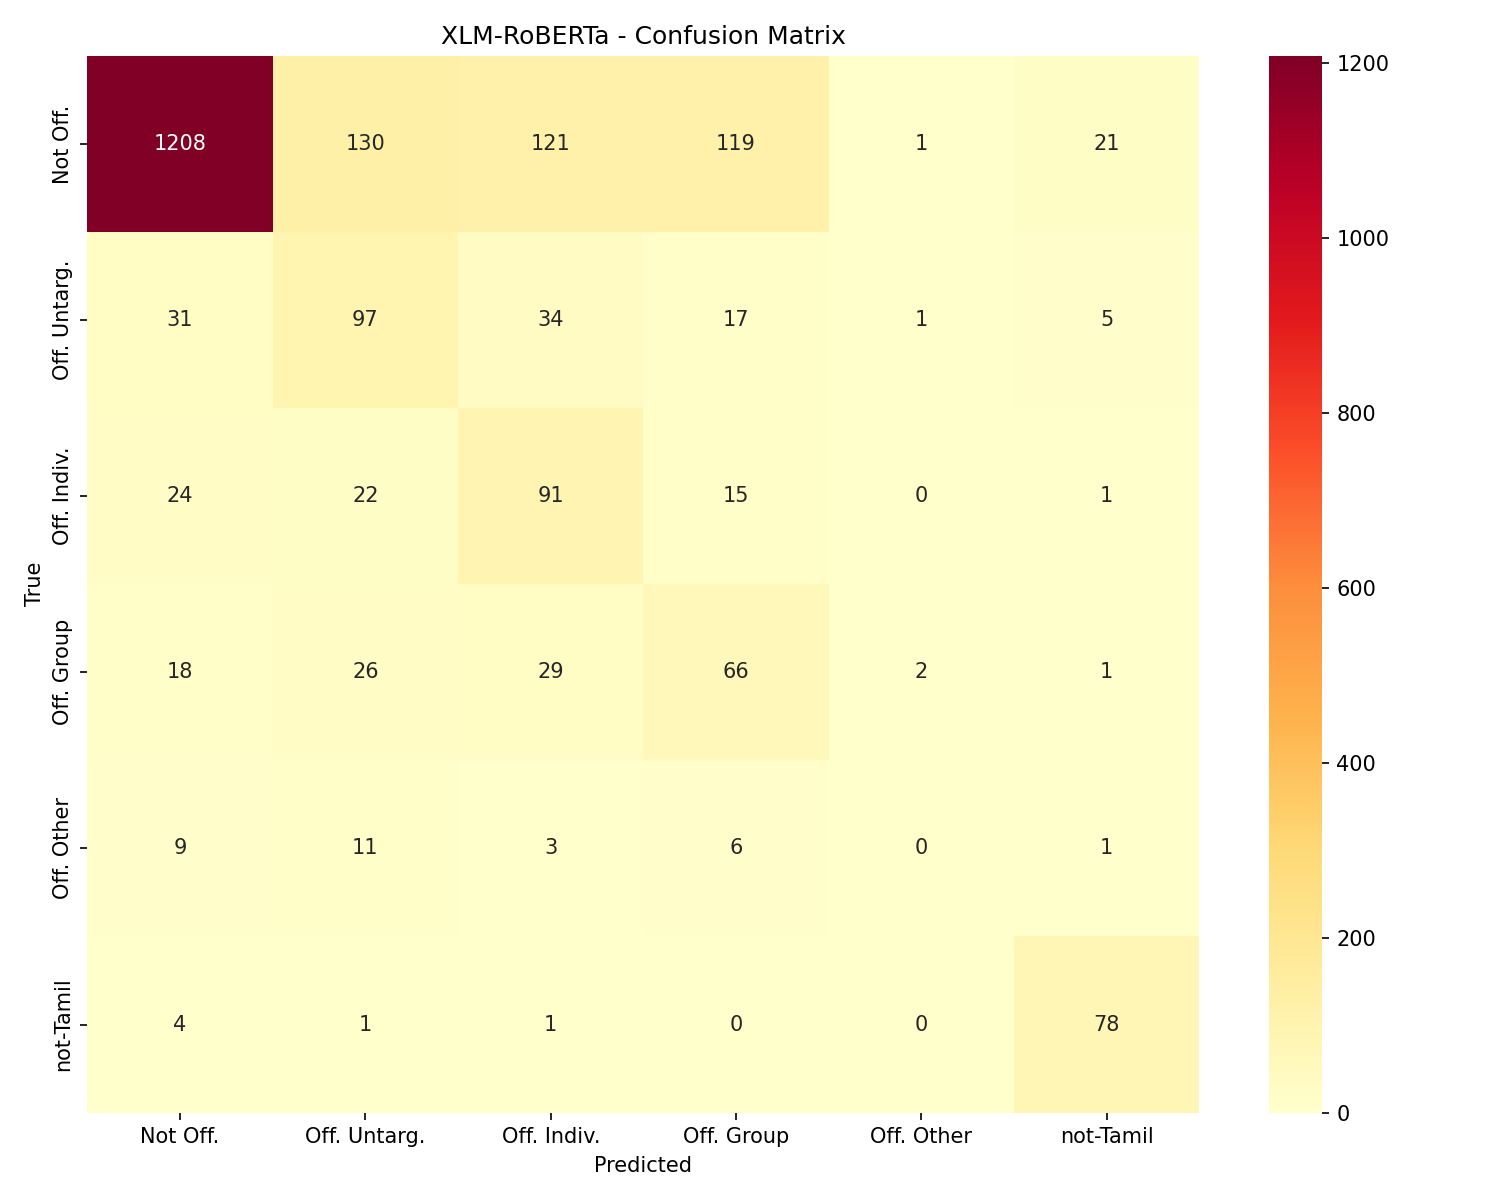
\includegraphics[width=\textwidth]{figures/xlm-roberta_confusion_matrix.png}
    \caption{XLM-RoBERTa}
    \label{fig:cm_xlmr}
\end{subfigure}
\caption{Confusion matrices for (a) MuRIL and (b) XLM-RoBERTa on the test set.}
\label{fig:cm_both}
\end{figure}

Key observations from the confusion matrices include:

\begin{enumerate}[leftmargin=2em]
    \item The dominant diagonal for \texttt{Not\_offensive} confirms strong majority-class detection.
    \item Significant cross-category confusion exists between \texttt{Offensive\_Untargeted} and \texttt{Offensive\_Targeted\_Group}, likely because caste- and group-based offensive discourse often blurs the line between targeted and untargeted abuse.
    \item The \texttt{Offensive\_Targeted\_Other} row is almost entirely misclassified across all models, with most samples predicted as \texttt{Not\_offensive} or \texttt{Offensive\_Untargeted}.
    \item The \texttt{not-Tamil} class shows a clean, well-separated diagonal in all confusion matrices, confirming reliable language identification.
\end{enumerate}

\subsection{Training Dynamics}

Figure~\ref{fig:training_analysis} presents the validation F1-score trajectory during training and the training time comparison across models.

\begin{figure}[!htbp]
\centering
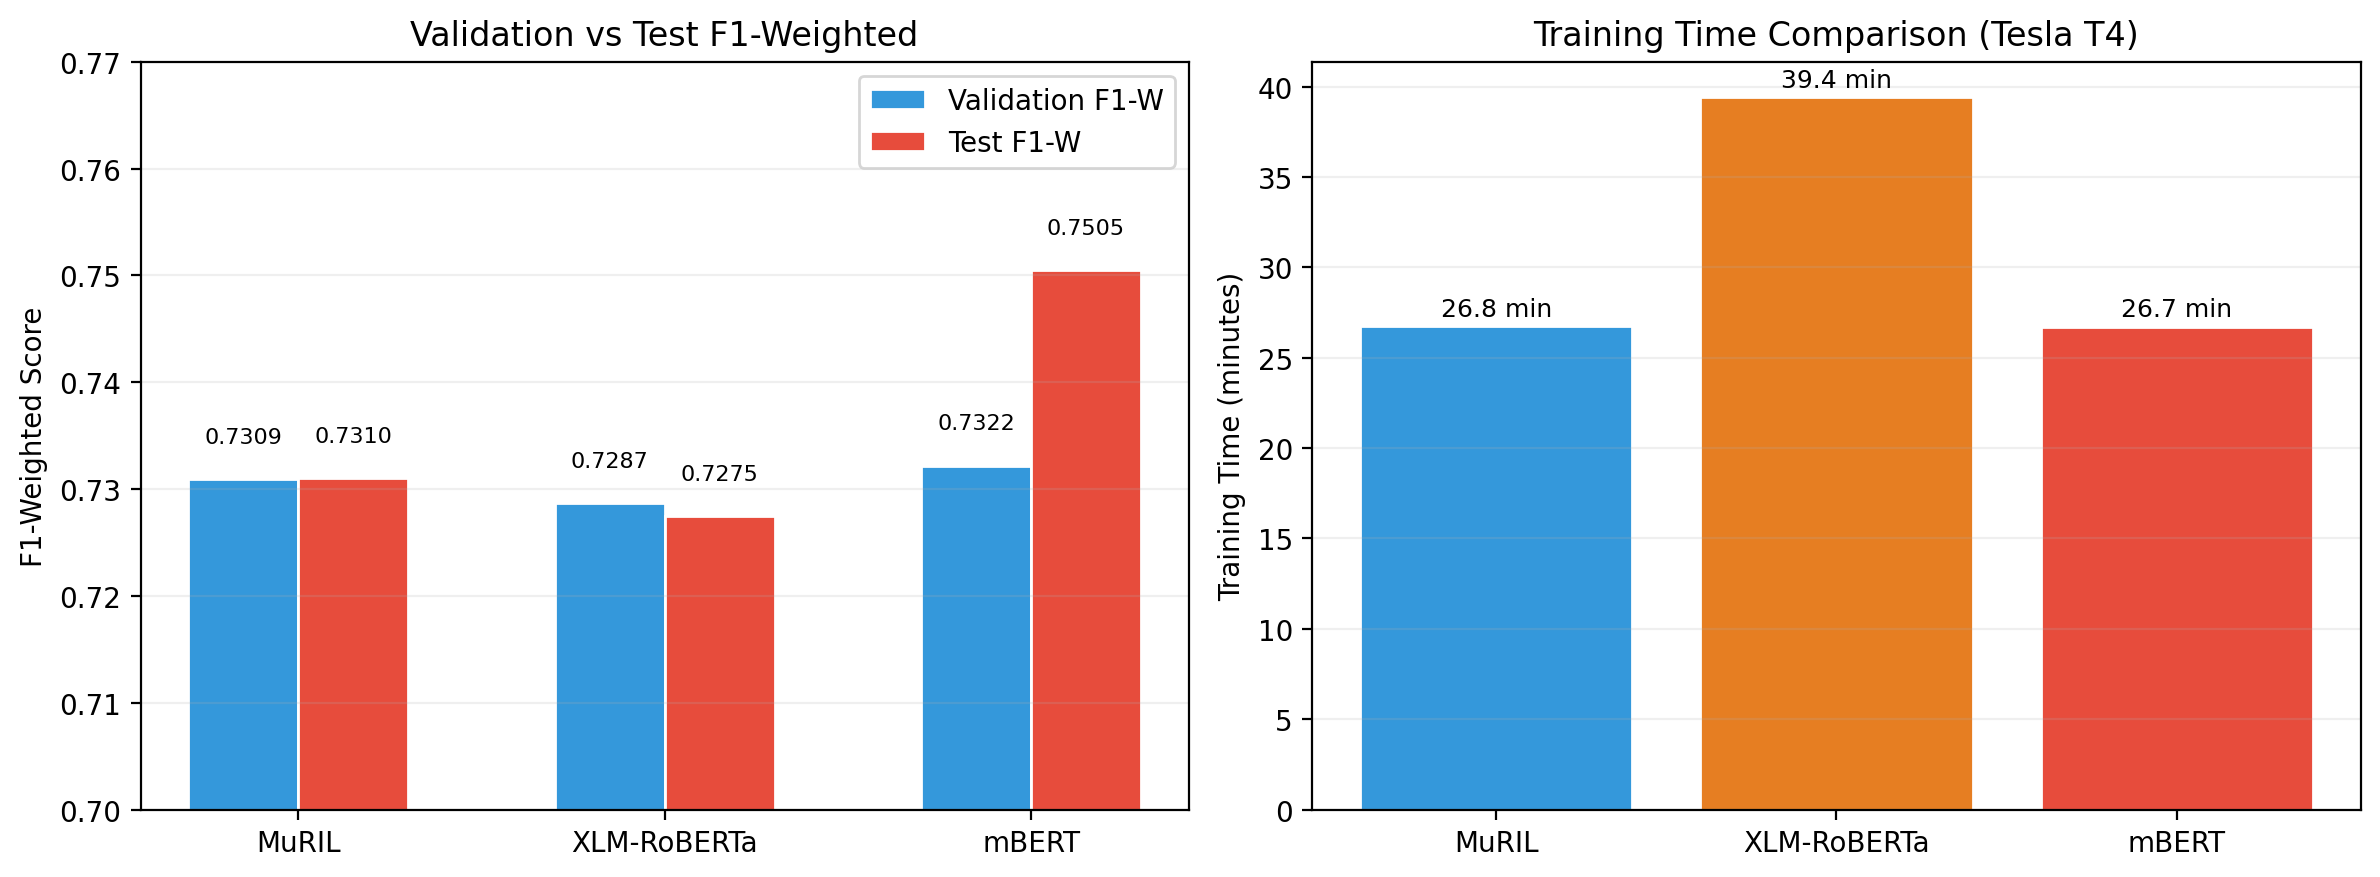
\includegraphics[width=0.85\textwidth]{figures/training_analysis.png}
\caption{Left: Validation F1-Weighted versus test F1-Weighted, revealing a gap for MuRIL (highest validation F1 but lower test F1, suggesting mild overfitting). Right: Training time comparison on Tesla T4 GPU.}
\label{fig:training_analysis}
\end{figure}

\FloatBarrier

% ══════════════════════════════════════════════════════════════════════════════
\section{Error Analysis and Explainability}
\label{sec:error_analysis}
% ══════════════════════════════════════════════════════════════════════════════

\subsection{Error Categorisation}

We perform a detailed analysis of the 595 misclassified samples from the best individual model (mBERT), which corresponds to a 27.1\% error rate on the test set. We categorise these errors into four distinct types, summarised in Table~\ref{tab:error_categories}.

\begin{table}[!htbp]
\centering
\caption{Categorisation of the 595 errors from mBERT on the test set. False positives (non-offensive text flagged as offensive) are the dominant error type.}
\label{tab:error_categories}
\begin{tabular}{l r r p{5cm}}
\toprule
\textbf{Error Type} & \textbf{Count} & \textbf{\%} & \textbf{Description} \\
\midrule
False Positives        & 292 & 49.1 & Non-offensive text incorrectly flagged as offensive \\[0.5em]
Cross-Category         & 159 & 26.7 & Misclassification between offensive sub-types \\[0.5em]
False Negatives        & 94  & 15.8 & Offensive text escaping detection (dangerous) \\[0.5em]
not-Tamil Errors       & 50  & 8.4  & Errors involving language identification \\
\bottomrule
\end{tabular}
\end{table}

\vspace{1em}

\textbf{False Positives (292 cases, 49.1\%):} This is the largest error category, and it has significant practical implications. When deployed for content moderation, a high false positive rate means that non-offensive content is wrongly censored, leading to user frustration and potential suppression of legitimate speech. Our analysis of these false positives reveals that they are predominantly driven by two factors: (a) aggressive but non-offensive fan discourse --- Tamil cinema fans frequently use emphatic, passionate language that employs aggressive-sounding words without being genuinely offensive; and (b) caste-community solidarity messages --- discussions about caste identity often use group-referencing language that the model associates with \texttt{Offensive\_Targeted\_Group}.

\textbf{Dangerous False Negatives (94 cases, 15.8\%):} These are the most critical errors from a content moderation perspective: offensive text that escapes automated detection. These cases would appear in users' feeds unfiltered, potentially causing harm. Many of these false negatives involve subtle, contextual offensiveness --- insults that rely on cultural knowledge, sarcastic remarks that superficially resemble neutral statements, or code-mixed offensive expressions where the offensive word is in one language and the context is in another.

\textbf{Cross-Category Confusion (159 cases, 26.7\%):} These errors involve misclassification between offensive sub-types (e.g., predicting \texttt{Offensive\_Untargeted} when the true label is \texttt{Offensive\_Targeted\_Group}). While these errors are less consequential than false negatives (the content is still identified as offensive, just miscategorised), they reduce the granularity of content moderation and hinder targeted intervention.

\textbf{not-Tamil Errors (50 cases, 8.4\%):} These errors involve the \texttt{not-Tamil} language identification class. Most are Hindi or Telugu comments that are misclassified as Tamil offensive content, likely because shared Devanagari or Latin-script tokens confuse the model.

\subsection{LIME Explainability Analysis}

We apply LIME to representative samples from the mBERT model to understand which linguistic features drive individual predictions. Figure~\ref{fig:lime} presents three illustrative examples.

\begin{figure}[!htbp]
\centering
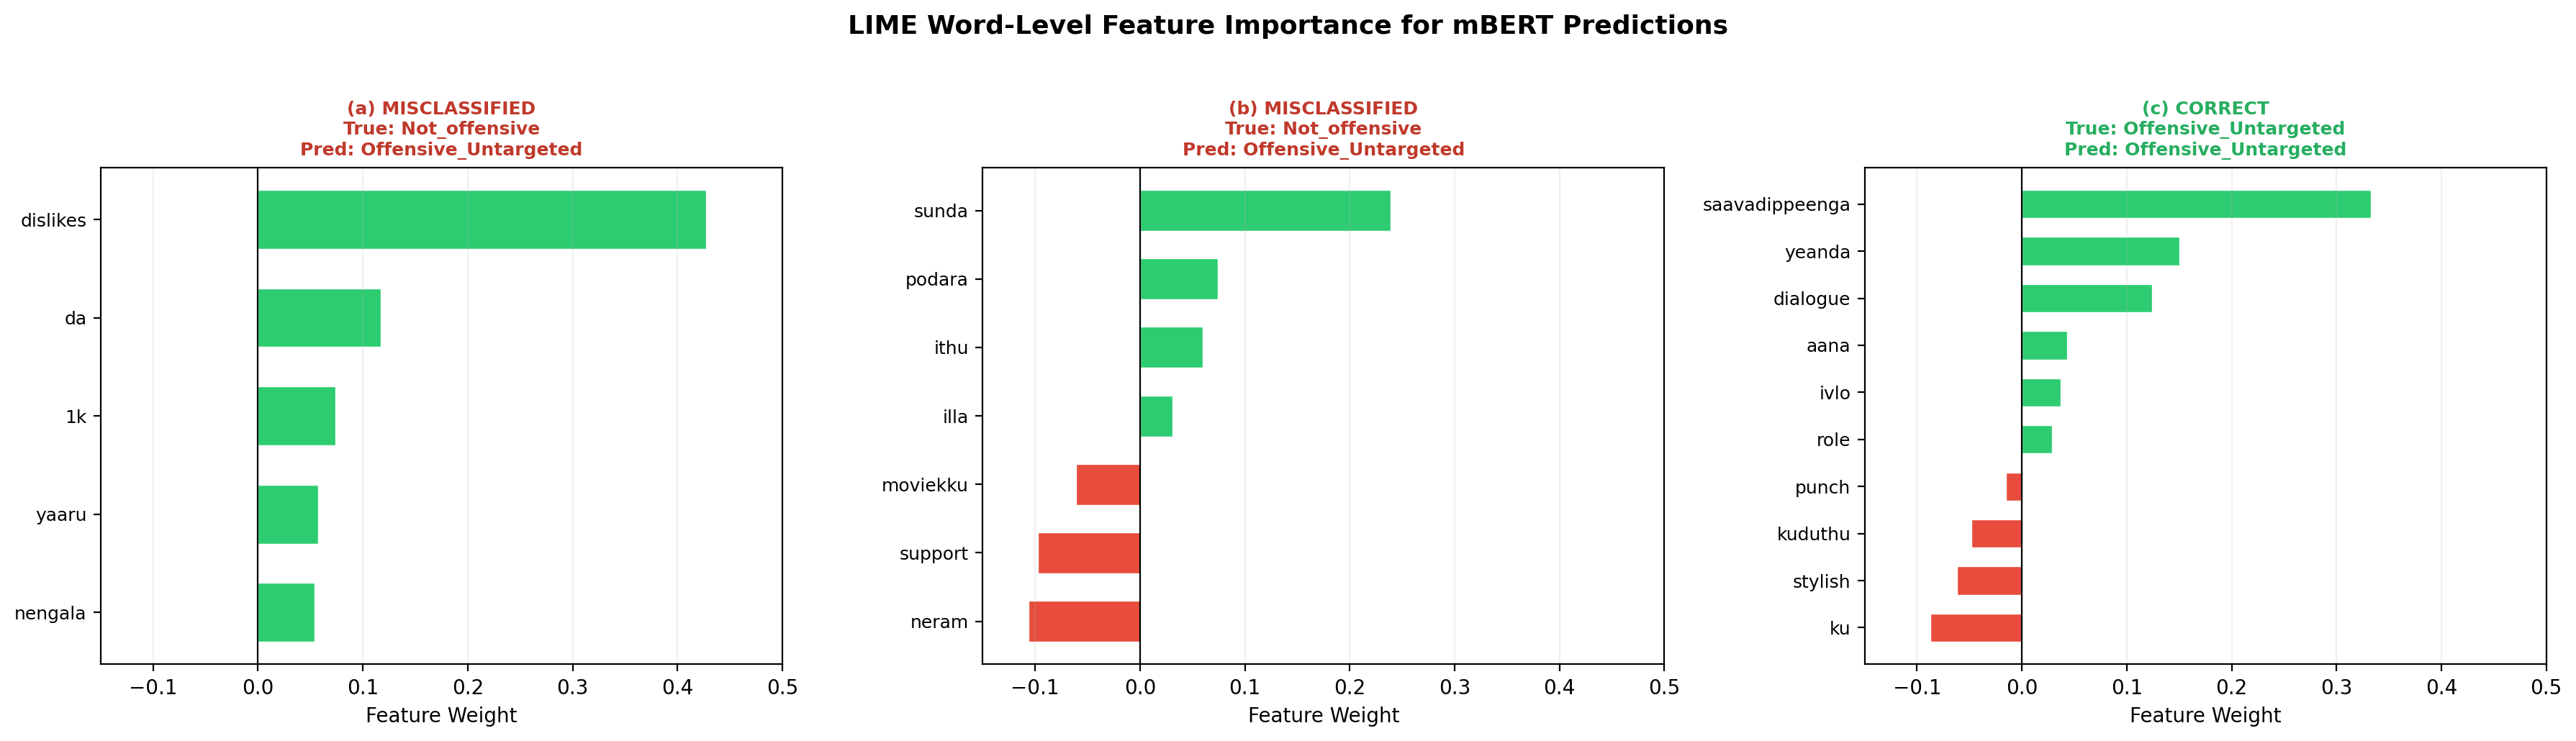
\includegraphics[width=0.95\textwidth]{figures/lime_explanations.png}
\caption{LIME word-level feature importance for three mBERT predictions. Green bars indicate features supporting the predicted class; red bars indicate features opposing it. (a, b) Misclassified samples where aggressive-sounding but non-offensive words trigger false positive predictions. (c) Correctly classified offensive sample where Tamil profanity is the dominant feature.}
\label{fig:lime}
\end{figure}

\FloatBarrier

Our LIME analysis reveals several important patterns in how the model processes Tamil and code-mixed text:

\textbf{Pattern 1 --- Legitimate offensive cues:} When the model correctly identifies offensive content, the LIME attributions typically highlight genuine offensive indicators. For example, the Tamil word ``\textit{saavadippeenga}'' (roughly translating to ``you'll be killed'' or ``you'll be beaten'') receives the highest positive attribution weight of 0.333, correctly driving the model toward an offensive prediction. This suggests that the model has successfully learned meaningful offensive vocabulary from the training data.

\textbf{Pattern 2 --- Spurious correlations with negative-sentiment English words:} In one misclassified sample, the English word ``dislikes'' receives the highest attribution weight of 0.427, triggering a false positive prediction of \texttt{Offensive\_Untargeted} for a comment that merely discusses YouTube video metrics (``\textit{1k dislikes yaaru da nengala}'' --- ``Who are you people giving 1k dislikes?''). This reveals a concerning spurious correlation: the model has learned to associate negative-sentiment English words with offensiveness, regardless of whether the word is being used in an offensive context.

\textbf{Pattern 3 --- Context-insensitive slang detection:} The Tamil colloquial word ``\textit{sunda}'' (meaning ``nothing'' or ``useless'' in casual speech) receives a high positive attribution (0.239), triggering an offensive prediction for a casual, non-offensive comment. This illustrates the model's inability to distinguish between casual Tamil slang and genuinely offensive language --- a distinction that requires deep cultural and contextual understanding.

\textbf{Pattern 4 --- Opposing features being overridden:} In several misclassified samples, words that correctly oppose the offensive prediction (e.g., ``support,'' ``neram'' meaning ``time'') receive negative LIME weights, but their influence is overridden by stronger spurious positive signals. This suggests that the model's decision boundary is dominated by a small number of high-weight lexical features, making it brittle when those features appear in non-offensive contexts.

These findings echo the observations of \citet{mathew2021hatexplain} regarding spurious correlations in English hate speech models, and suggest that analogous problems persist --- and may be amplified --- in code-mixed, low-resource language settings where training data is limited and lexical diversity is high.

% ══════════════════════════════════════════════════════════════════════════════
\section{Discussion}
\label{sec:discussion}
% ══════════════════════════════════════════════════════════════════════════════

\subsection{MuRIL versus General Multilingual Models: A Nuanced Picture}

One of the central questions motivating this study was whether Indian-language-specific pre-training (MuRIL) would outperform general multilingual pre-training (XLM-RoBERTa, mBERT) for Tamil offensive language detection. Our results paint a nuanced picture that defies a simple yes-or-no answer.

On the one hand, MuRIL does not achieve the best \textit{overall} test-set performance. Its weighted F1-score of 0.7310 lags behind mBERT's 0.7505 by a margin of 1.95\% absolute. Its macro F1-score of 0.4405 is the lowest among the three models, indicating particularly poor performance on minority classes. These results suggest that Indian-language-specific pre-training alone is not a silver bullet for code-mixed social media text.

On the other hand, the per-script analysis (Table~\ref{tab:script_performance}) reveals that \textbf{MuRIL is the best individual model on pure Tamil Unicode text}, with a weighted F1-score of 0.771 --- 2.4\% higher than mBERT's 0.747. This confirms that MuRIL's Indian-language pre-training does provide genuine advantages for native-script content, where its deeper understanding of Tamil vocabulary, morphology, and semantics can be fully leveraged.

The resolution of this apparent contradiction lies in the \textit{composition of the dataset}: Latin-script (Tanglish) content constitutes 80\% of the test set, and mBERT's superiority on Tanglish text (0.749 vs.\ MuRIL's 0.719) drives its overall advantage. This suggests that MuRIL's transliteration-aware pre-training, while theoretically well-suited for Tanglish, may not fully capture the creative, non-standard spellings characteristic of YouTube Tanglish, which differs systematically from the more standard transliterations in MuRIL's pre-training data.

We caution that this finding is based on a single random seed and a single test split, and should be validated through multi-seed experiments with confidence intervals.

\subsection{Ensemble Trade-offs}

The majority-voting ensemble achieves the best weighted F1-score (0.7620), improving over mBERT by +1.15\% absolute, and the best accuracy (0.7502), improving by +2.14\% absolute. However, it slightly decreases the macro F1-score (0.4947 vs.\ mBERT's 0.4972), a difference of $-$0.25\%.

This trade-off is inherent to majority voting: when two out of three models predict the majority class (\texttt{Not\_offensive}), the ensemble follows, even if the third model correctly identifies a minority-class offensive sample. This ``majority-class amplification'' effect improves weighted metrics (which are dominated by the majority class) at the expense of minority-class macro metrics.

More sophisticated ensemble strategies --- such as weighted voting based on per-class F1-scores, stacking with a meta-learner, or probability averaging with calibrated confidence scores --- could potentially mitigate this trade-off, and we consider them promising directions for future work.

\subsection{The Challenge of Extreme Class Imbalance}

Class imbalance is the single most significant challenge in this study. Despite employing inverse-frequency class weighting, minority offensive sub-types remain extremely difficult to detect. The \texttt{Offensive\_Targeted\_Other} class, with only 454 training samples (1.3\%) and approximately 30 test samples, achieves an F1-score of 0.000 for all models except mBERT (0.082). Even the intermediate classes (\texttt{Untargeted}, \texttt{Targeted\_Individual}, \texttt{Targeted\_Group}) achieve F1-scores below 0.45.

This suggests that weighted cross-entropy alone is insufficient for extreme imbalance ratios. More aggressive strategies may be needed, including:

\begin{itemize}[leftmargin=2em]
    \item \textbf{Focal Loss} \citep{lin2017focal}: Down-weights the loss contribution from well-classified (easy) examples, focusing training on hard, misclassified samples. The focusing parameter $\gamma$ controls the degree of down-weighting.
    
    \item \textbf{Minority class oversampling:} Duplicating or synthetically augmenting training samples from underrepresented classes to create a more balanced training distribution.
    
    \item \textbf{Two-stage classification:} First classifying as ``offensive'' vs.\ ``not-offensive'' (a more balanced binary task), then sub-classifying offensive samples into specific categories.
    
    \item \textbf{Data augmentation:} Back-translation, synonym replacement, or generative augmentation to create additional training samples for minority classes.
\end{itemize}

\subsection{The False Positive Problem}

The predominance of false positives (292 cases, 49.1\% of all errors) over false negatives (94 cases, 15.8\%) reveals an important asymmetry: the model errs on the side of over-moderation rather than under-moderation. While this may seem preferable from a safety perspective (it is ``better'' to wrongly flag non-offensive content than to miss offensive content), excessive false positives in a deployed system lead to user frustration, erosion of trust, and --- in the worst case --- suppression of legitimate speech.

The root cause of many false positives is the model's conflation of \textit{aggressive linguistic style} with \textit{offensive intent}. Tamil cinema fan communities, for example, use highly emphatic, passionate, and sometimes combative language to express support for their favourite actors. Statements like ``\textit{mass da}'' (``it's awesome, man'') or ``\textit{vera level}'' (``another level'') employ aggressive-sounding words in entirely positive contexts, but the model --- having learned that such words frequently co-occur with offensive content --- incorrectly flags them.

Addressing this false positive problem likely requires going beyond purely lexical features and incorporating discourse-level context, pragmatic intent recognition, and cultural knowledge --- all of which are challenging research frontiers for low-resource language NLP.

\subsection{Limitations}

We acknowledge several limitations of this study:

\begin{enumerate}[leftmargin=2em]
    \item \textbf{Single random seed:} All experiments use a single random initialisation (seed=42). Transformer fine-tuning is known to be sensitive to random seeds, and results may vary by 1--3\% F1 across different initialisations. Multi-seed experiments with bootstrap confidence intervals are needed to establish the statistical significance of observed differences.
    
    \item \textbf{Custom test split:} Our test set is derived from the original validation set, not the official shared task test set. This limits direct comparability with published shared task results and introduces the risk that our test set may not be representative of the broader distribution.
    
    \item \textbf{Platform specificity:} The dataset consists exclusively of YouTube comments. Offensive language on Twitter/X, WhatsApp, Facebook, and other platforms may differ in style, length, and code-mixing patterns, limiting the generalisability of our findings.
    
    \item \textbf{Limited explainability scope:} Our LIME analysis covers only a small number of qualitative examples. A comprehensive quantitative explainability evaluation (e.g., faithfulness, sufficiency, and comprehensiveness metrics as in \citet{mathew2021hatexplain}) is needed but was beyond the scope of this study.
    
    \item \textbf{Single language focus:} While the OffensEval Dravidian dataset also includes Malayalam and Kannada, this study focuses exclusively on Tamil. Cross-lingual and multilingual experiments across Dravidian languages are planned as future work.
    
    \item \textbf{Single imbalance strategy:} Only weighted cross-entropy is explored. Focal loss, oversampling, and hybrid strategies may yield significantly better minority-class detection.
\end{enumerate}

\FloatBarrier

% ══════════════════════════════════════════════════════════════════════════════
\section{Ethical Considerations}
\label{sec:ethics}
% ══════════════════════════════════════════════════════════════════════════════

This work involves the processing and analysis of offensive and potentially harmful language content, including caste-based slurs, targeted abuse, and profanity. We acknowledge several ethical dimensions:

\begin{enumerate}[leftmargin=2em]
    \item \textbf{Annotator welfare:} The OffensEval Dravidian dataset was created by external researchers \citep{chakravarthi2021dataset}; we did not perform annotation ourselves. However, we recognise that exposure to large volumes of offensive content during annotation can cause psychological harm to annotators, and urge future data collection efforts to implement appropriate support mechanisms.
    
    \item \textbf{Dual-use concerns:} Automated offensive language detection systems can be repurposed for censorship, political suppression, or the silencing of legitimate dissent. This is a particular concern in politically sensitive contexts, and we urge that any deployment of such systems be accompanied by robust appeals mechanisms and human oversight.
    
    \item \textbf{Bias amplification:} The model inherits and potentially amplifies biases present in the training data. The high false positive rate on caste-community messages suggests that the model may disproportionately flag content from certain communities, raising fairness concerns. Systematic bias auditing is essential before deployment.
    
    \item \textbf{Cultural sensitivity:} Offensiveness is inherently contextual, subjective, and culturally dependent. A model trained on Tamil YouTube data should not be deployed for other Tamil-speaking communities (e.g., Sri Lankan Tamil, Singapore Tamil) without re-evaluation, as cultural norms around offensive language may differ significantly.
\end{enumerate}

\FloatBarrier

% ══════════════════════════════════════════════════════════════════════════════
\section{Conclusion and Future Work}
\label{sec:conclusion}
% ══════════════════════════════════════════════════════════════════════════════

This paper has presented a comprehensive comparative study of three multilingual transformer models --- MuRIL, XLM-RoBERTa, and mBERT --- for the task of offensive language detection in Tamil and code-mixed Tamil-English (Tanglish) social media text. Through systematic experimentation on the OffensEval Dravidian dataset, ensemble learning, and LIME-based explainability analysis, we have arrived at several key findings that contribute to both the theoretical understanding and practical development of offensive language detection systems for low-resource Dravidian languages.

Our principal findings can be summarised as follows:

\begin{enumerate}[leftmargin=2em]
    \item \textbf{mBERT achieves the best individual performance} (F1-W: 0.7505), outperforming both MuRIL (0.7310) and XLM-RoBERTa (0.7275) on the overall test set. This somewhat counterintuitive result is driven by mBERT's superior handling of Latin-script Tanglish text, which dominates the dataset.
    
    \item \textbf{Indian-language-specific pre-training provides script-dependent advantages.} MuRIL is the strongest individual model on pure Tamil Unicode text (F1-W: 0.771), confirming that Indian-language pre-training helps for native-script content. However, its weaker Tanglish performance limits its overall effectiveness on this Tanglish-dominated dataset.
    
    \item \textbf{Majority-voting ensemble improves weighted performance} (F1-W: 0.7620, +1.15\% over mBERT), winning on 4 out of 6 classes. The three models capture complementary linguistic signals, validating the diversity-based ensemble approach.
    
    \item \textbf{Class imbalance remains the dominant challenge.} Despite weighted cross-entropy loss, the rarest class (\texttt{Offensive\_Targeted\_Other}, 1.3\% of training data) achieves near-zero F1 across all approaches, and intermediate offensive sub-categories remain below 0.45 F1.
    
    \item \textbf{LIME analysis reveals both legitimate cues and spurious correlations.} The model correctly learns Tamil profanity as offensive indicators but also associates negative-sentiment English words (e.g., ``dislikes'') with offensiveness regardless of context.
    
    \item \textbf{False positives dominate the error landscape} (49.1\% of all errors), primarily driven by aggressive but non-offensive fan discourse and caste-community solidarity messages.
\end{enumerate}

\subsection{Future Directions}

Building on the findings and limitations of this study, we identify several promising directions for future research:

\begin{enumerate}[leftmargin=2em]
    \item \textbf{Advanced class imbalance strategies:} Exploring Focal Loss \citep{lin2017focal}, synthetic minority oversampling (SMOTE), generative data augmentation (e.g., using large language models to generate minority-class samples), and two-stage classification pipelines.
    
    \item \textbf{Multi-seed experiments:} Conducting experiments across multiple random seeds (e.g., 5--10 seeds) with bootstrap confidence intervals to establish the statistical significance of observed performance differences.
    
    \item \textbf{Cross-lingual Dravidian experiments:} Extending the study to Malayalam and Kannada from the OffensEval Dravidian dataset, and investigating zero-shot and few-shot cross-lingual transfer between Dravidian languages.
    
    \item \textbf{Learned ensemble methods:} Replacing majority voting with weighted voting (based on per-class F1-scores), probability averaging, or stacking with a meta-learner to better handle minority classes.
    
    \item \textbf{Quantitative explainability benchmarks:} Developing or adapting explainability evaluation metrics (faithfulness, sufficiency, comprehensiveness) for code-mixed Tamil text, building on the HateXplain framework \citep{mathew2021hatexplain}.
    
    \item \textbf{Cultural context modelling:} Incorporating external knowledge sources (e.g., Tamil slang dictionaries, fan community terminology databases) to help models distinguish between aggressive-but-non-offensive and genuinely offensive language.
    
    \item \textbf{Real-time deployment:} Developing a deployable content moderation API with latency-optimised inference, human-in-the-loop review mechanisms, and support for multiple Indian languages.
\end{enumerate}

\subsection{Code and Data Availability}

Our complete implementation, including all training, evaluation, error analysis, and explainability scripts, is publicly available at \url{https://github.com/naveen-231006/Hate-Word}. The OffensEval Dravidian dataset is publicly available via HuggingFace Datasets \citep{chakravarthi2021dataset}.

\FloatBarrier

% ══════════════════════════════════════════════════════════════════════════════
% REFERENCES
% ══════════════════════════════════════════════════════════════════════════════

\bibliographystyle{plainnat}

\begin{thebibliography}{30}

\bibitem[IAMAI(2025)]{iamai2025}
Internet and Mobile Association of India.
\newblock India Internet Report 2025.
\newblock Technical report, IAMAI, 2025.

\bibitem[Fortuna and Nunes(2018)]{fortuna2018survey}
P.~Fortuna and S.~Nunes.
\newblock A survey on automatic detection of hate speech in text.
\newblock \textit{ACM Computing Surveys}, 51(4):1--30, 2018.

\bibitem[Schmidt and Wiegand(2017)]{schmidt2017survey}
A.~Schmidt and M.~Wiegand.
\newblock A survey on hate speech detection using natural language processing.
\newblock In \textit{Proc.\ SocialNLP Workshop at EACL}, pages 1--10, 2017.

\bibitem[Davidson et~al.(2017)]{davidson2017automated}
T.~Davidson, D.~Warmsley, M.~Macy, and I.~Weber.
\newblock Automated hate speech detection and the problem of offensive language.
\newblock In \textit{Proc.\ ICWSM}, pages 512--515, 2017.

\bibitem[Waseem and Hovy(2016)]{waseem2016hateful}
Z.~Waseem and D.~Hovy.
\newblock Hateful symbols or hateful people? Predictive features for hate speech detection on Twitter.
\newblock In \textit{Proc.\ NAACL Student Research Workshop}, pages 88--93, 2016.

\bibitem[Badjatiya et~al.(2017)]{badjatiya2017deep}
P.~Badjatiya, S.~Gupta, M.~Gupta, and V.~Varma.
\newblock Deep learning for hate speech detection in tweets.
\newblock In \textit{Proc.\ WWW Companion}, pages 759--760, 2017.

\bibitem[Vaswani et~al.(2017)]{vaswani2017attention}
A.~Vaswani, N.~Shazeer, N.~Parmar, J.~Uszkoreit, L.~Jones, A.~N.~Gomez, \L.~Kaiser, and I.~Polosukhin.
\newblock Attention is all you need.
\newblock In \textit{Advances in Neural Information Processing Systems}, pages 5998--6008, 2017.

\bibitem[Devlin et~al.(2019)]{devlin2019bert}
J.~Devlin, M.-W.~Chang, K.~Lee, and K.~Toutanova.
\newblock {BERT}: Pre-training of deep bidirectional transformers for language understanding.
\newblock In \textit{Proc.\ NAACL-HLT}, pages 4171--4186, 2019.

\bibitem[Conneau et~al.(2020)]{conneau2020xlmr}
A.~Conneau, K.~Khandelwal, N.~Goyal, V.~Chaudhary, G.~Wenzek, F.~Guzm{\'a}n, E.~Grave, M.~Ott, L.~Zettlemoyer, and V.~Stoyanov.
\newblock Unsupervised cross-lingual representation learning at scale.
\newblock In \textit{Proc.\ ACL}, pages 8440--8451, 2020.

\bibitem[Liu et~al.(2019)]{liu2019roberta}
Y.~Liu, M.~Ott, N.~Goyal, J.~Du, M.~Joshi, D.~Chen, O.~Levy, M.~Lewis, L.~Zettlemoyer, and V.~Stoyanov.
\newblock {RoBERTa}: A robustly optimized {BERT} pretraining approach.
\newblock \textit{arXiv preprint arXiv:1907.11692}, 2019.

\bibitem[Khanuja et~al.(2021)]{khanuja2021muril}
S.~Khanuja, D.~Bansal, S.~Mehtani, S.~Khapra, D.~Ganapathy, G.~Sagare, C.~McKeown, J.~Sessi, R.~Gupta, and P.~Shah.
\newblock {MuRIL}: Multilingual Representations for Indian Languages.
\newblock In \textit{Findings of ACL}, pages 3929--3936, 2021.

\bibitem[Caselli et~al.(2021)]{caselli2021hatebert}
T.~Caselli, V.~Basile, J.~Mitrovi{\'c}, and M.~Granitzer.
\newblock {HateBERT}: Retraining {BERT} for abusive language detection in English.
\newblock In \textit{Proc.\ WOAH Workshop at ACL}, pages 17--25, 2021.

\bibitem[Mathew et~al.(2021)]{mathew2021hatexplain}
B.~Mathew, P.~Saha, S.~M.~Yimam, C.~Biemann, P.~Goyal, and A.~Mukherjee.
\newblock {HateXplain}: A benchmark dataset for explainable hate speech detection.
\newblock In \textit{Proc.\ AAAI}, pages 14867--14875, 2021.

\bibitem[Pires et~al.(2019)]{pires2019multilingual}
T.~Pires, E.~Schlinger, and D.~Garrette.
\newblock How multilingual is multilingual {BERT}?
\newblock In \textit{Proc.\ ACL}, pages 4996--5001, 2019.

\bibitem[Pamungkas and Patti(2019)]{pamungkas2019cross}
E.~W.~Pamungkas and V.~Patti.
\newblock Cross-domain and cross-lingual abusive language detection: A hybrid approach with deep learning and a multilingual lexicon.
\newblock In \textit{Proc.\ ACL Student Research Workshop}, pages 363--370, 2019.

\bibitem[Chakravarthi et~al.(2021a)]{chakravarthi2021dravidian}
B.~R.~Chakravarthi, R.~Priyadharshini, V.~Muralidaran, N.~Jose, S.~Suryawanshi, E.~Sherly, and J.~P.~McCrae.
\newblock Findings of the shared task on offensive language identification in Tamil, Malayalam, and Kannada.
\newblock In \textit{Proc.\ DravidianLangTech Workshop at EACL}, 2021.

\bibitem[Chakravarthi et~al.(2021b)]{chakravarthi2021dataset}
B.~R.~Chakravarthi, R.~Priyadharshini, R.~Jose, M.~Kumar, S.~Suryawanshi, E.~Sherly, and J.~P.~McCrae.
\newblock Dataset for identification of homophobia and transphobia in multilingual YouTube comments.
\newblock \textit{arXiv preprint arXiv:2109.00227}, 2021.

\bibitem[Dowlagar and Mamidi(2021)]{dowlagar2021cfilt}
S.~Dowlagar and R.~Mamidi.
\newblock {CfiltIITB} at {DravidianLangTech@EACL2021}: Offensive language identification in Dravidian languages.
\newblock In \textit{Proc.\ DravidianLangTech Workshop at EACL}, 2021.

\bibitem[Risch et~al.(2020)]{risch2020data}
J.~Risch, R.~Krestel, et~al.
\newblock Data augmentation for cross-domain hate speech detection.
\newblock \textit{arXiv preprint arXiv:2004.10404}, 2020.

\bibitem[Rajamanickam et~al.(2020)]{rajamanickam2020joint}
S.~Rajamanickam, P.~Mishra, H.~Yannakoudakis, and E.~Shutova.
\newblock Joint multitask learning for community question answering using task-specific embeddings.
\newblock In \textit{Proc.\ EMNLP}, 2020.

\bibitem[Bali et~al.(2014)]{bali2014borrowing}
K.~Bali, J.~Sharma, M.~Choudhury, and Y.~Vyas.
\newblock ``{I} am borrowing ya mixing?'': An analysis of {English-Hindi} code mixing in {Facebook}.
\newblock In \textit{Proc.\ Workshop on Computational Approaches to Code Switching at EMNLP}, pages 116--126, 2014.

\bibitem[Subramanian et~al.(2022)]{subramanian2022phrase}
M.~Subramanian, V.~E.~Sathiskumar, G.~Deepalakshmi, J.~Cho, and G.~Manikandan.
\newblock The effect of phrase vector embedding in explainable hierarchical attention-based Tamil code-mixed hate speech and intent detection.
\newblock \textit{Electronics}, 11(24):4175, 2022.

\bibitem[Ribeiro et~al.(2016)]{ribeiro2016lime}
M.~T.~Ribeiro, S.~Singh, and C.~Guestrin.
\newblock ``{Why} should {I} trust you?'': Explaining the predictions of any classifier.
\newblock In \textit{Proc.\ KDD}, pages 1135--1144, 2016.

\bibitem[Lundberg and Lee(2017)]{lundberg2017shap}
S.~M.~Lundberg and S.-I.~Lee.
\newblock A unified approach to interpreting model predictions.
\newblock In \textit{Advances in Neural Information Processing Systems}, pages 4765--4774, 2017.

\bibitem[Lin et~al.(2017)]{lin2017focal}
T.-Y.~Lin, P.~Goyal, R.~Girshick, K.~He, and P.~Doll{\'a}r.
\newblock Focal loss for dense object detection.
\newblock In \textit{Proc.\ ICCV}, pages 2980--2988, 2017.

\end{thebibliography}

\end{document}
